$\alpha = \beta = 1$ and $t_f= 0$.
Now we simulate our system for $H = 1I, 10I, 100I$ and plot $K(t)$ matrix, $u(t)$ and states of system.

\begin{itemize}
	%%%%%%%%% H = 1I %%%%%%%%%
	\item $H = 1I$
	\begin{figure}[H]
		\caption{$K(t)$ in $H = 1I$}
		\centering
		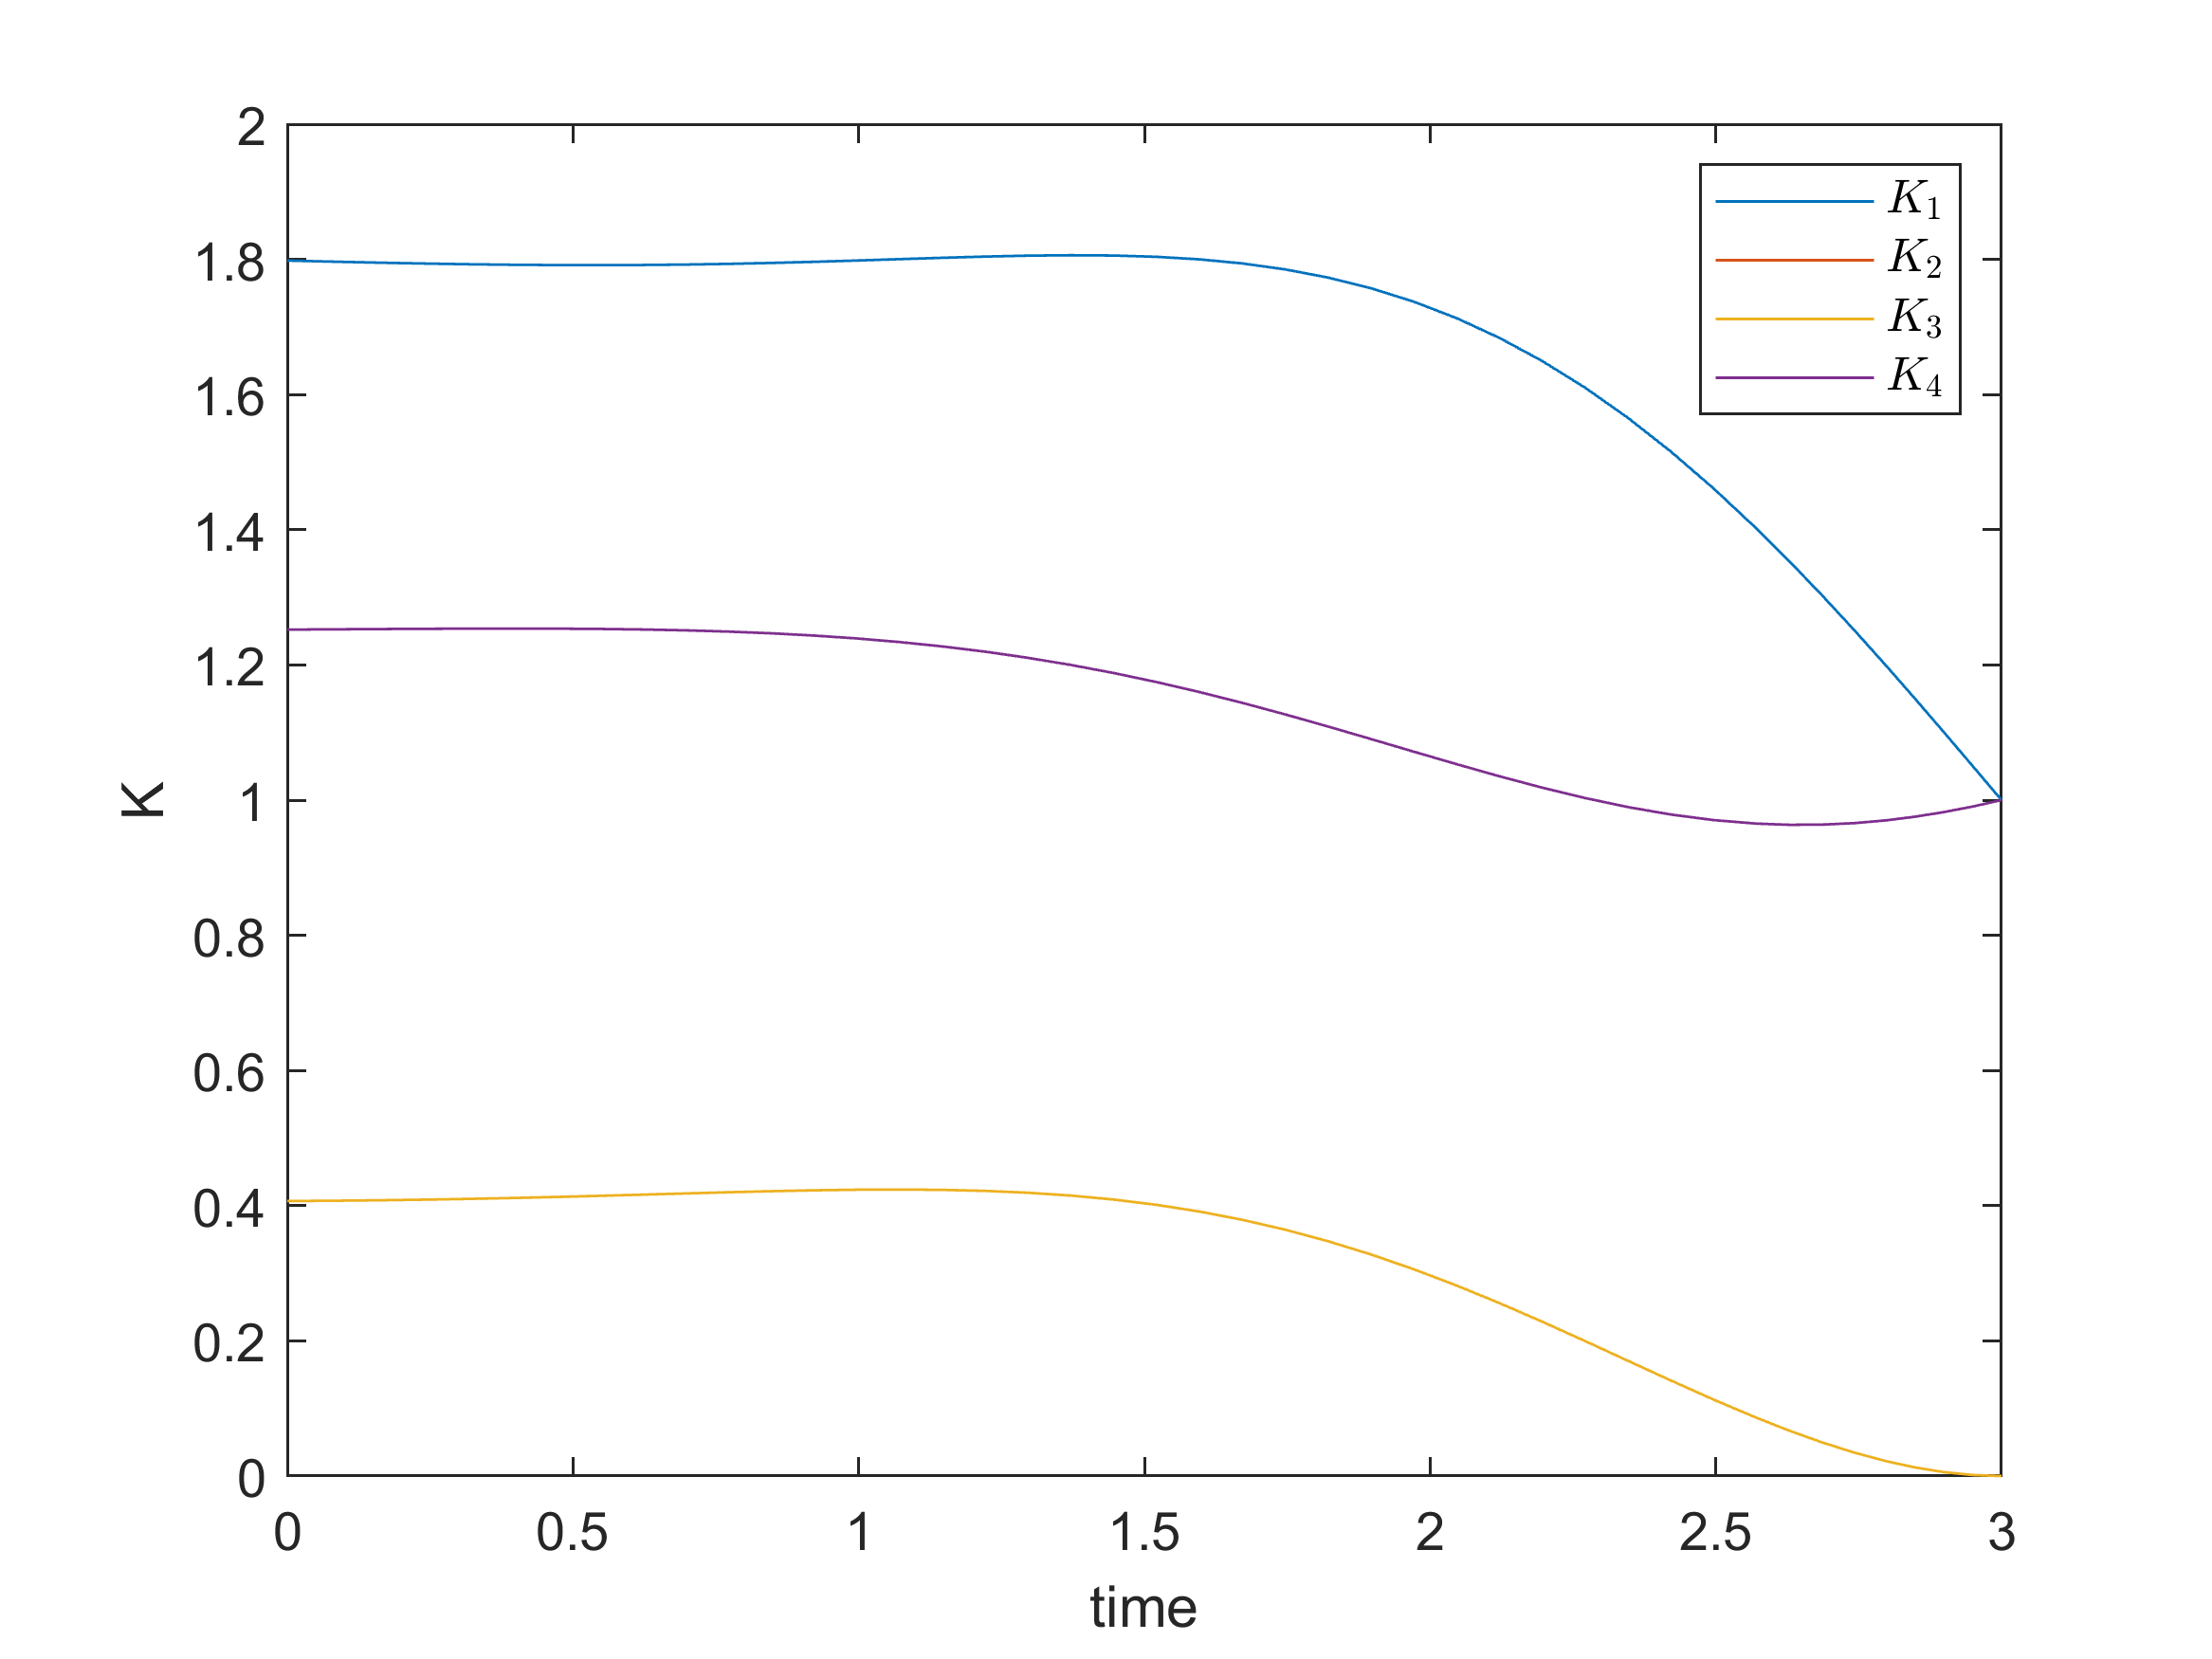
\includegraphics[width=12cm]{../Code/Q3/figures/KH1.png}
	\end{figure}
\begin{figure}[H]
	\caption{$u(t)$ in $H = 1I$}
	\centering
	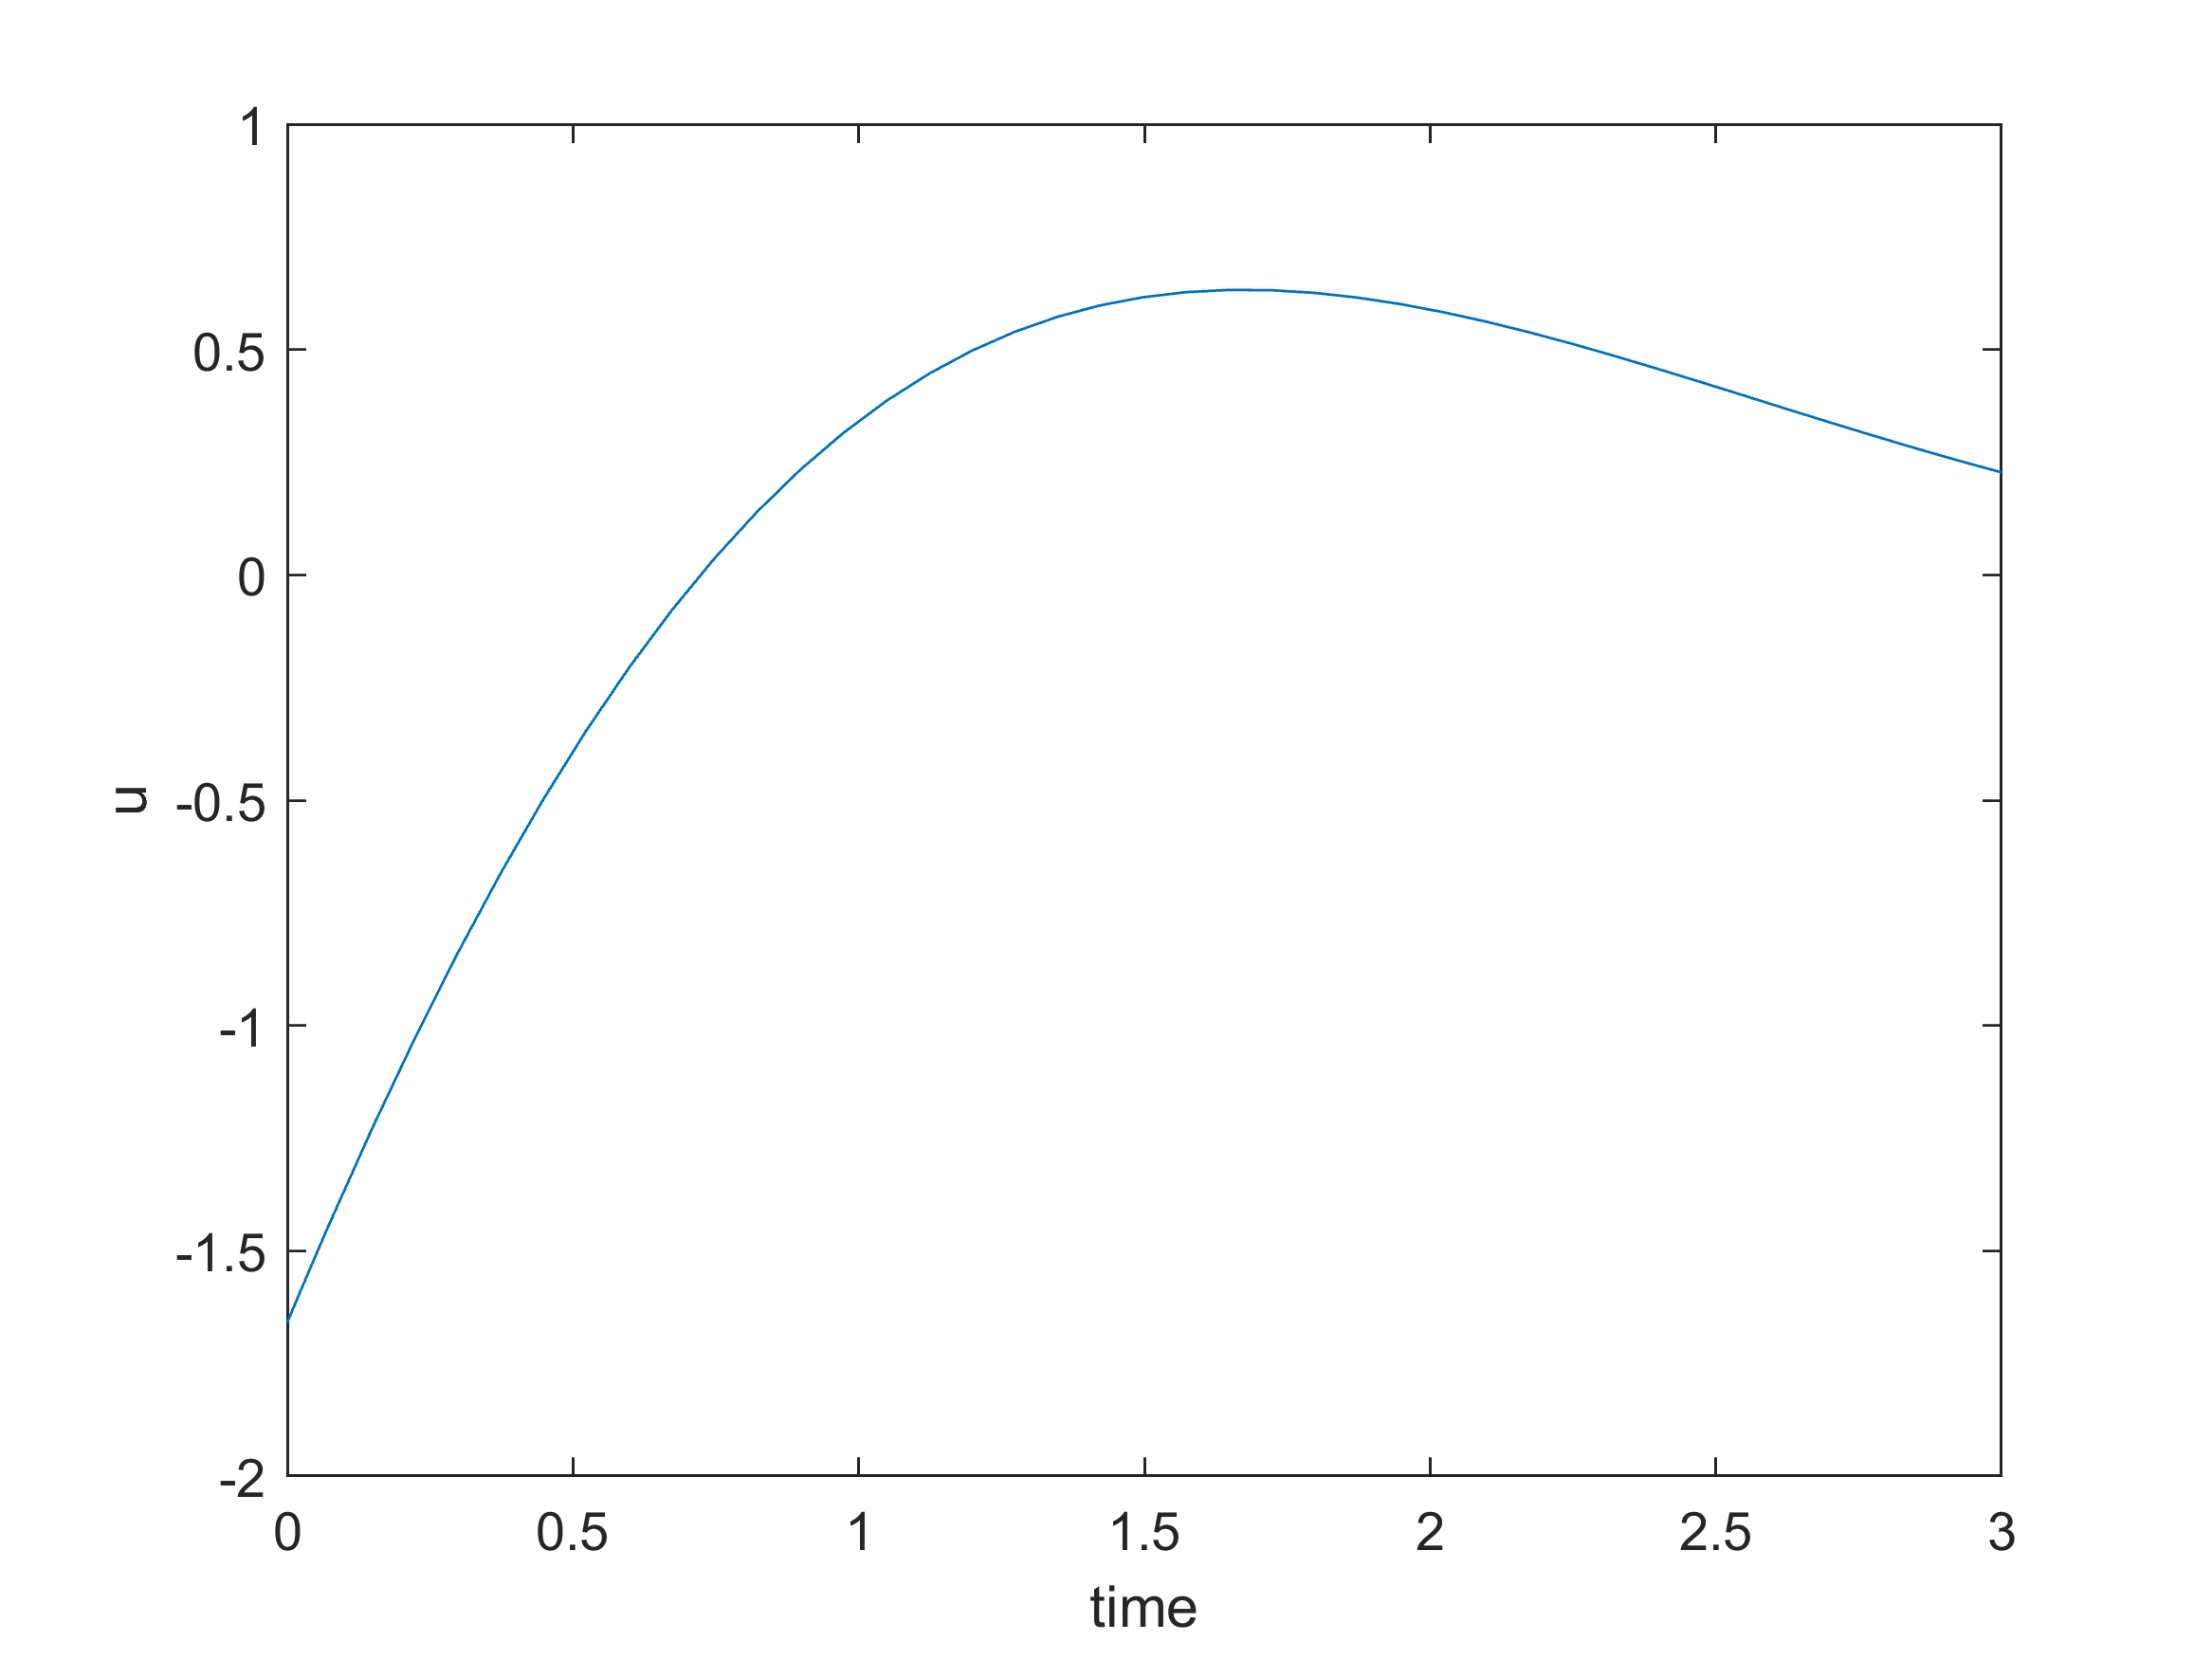
\includegraphics[width=12cm]{../Code/Q3/figures/uH1.png}
\end{figure}
\begin{figure}[H]
	\caption{System States $\vec x(t)$ in $H = 1I$}
	\centering
	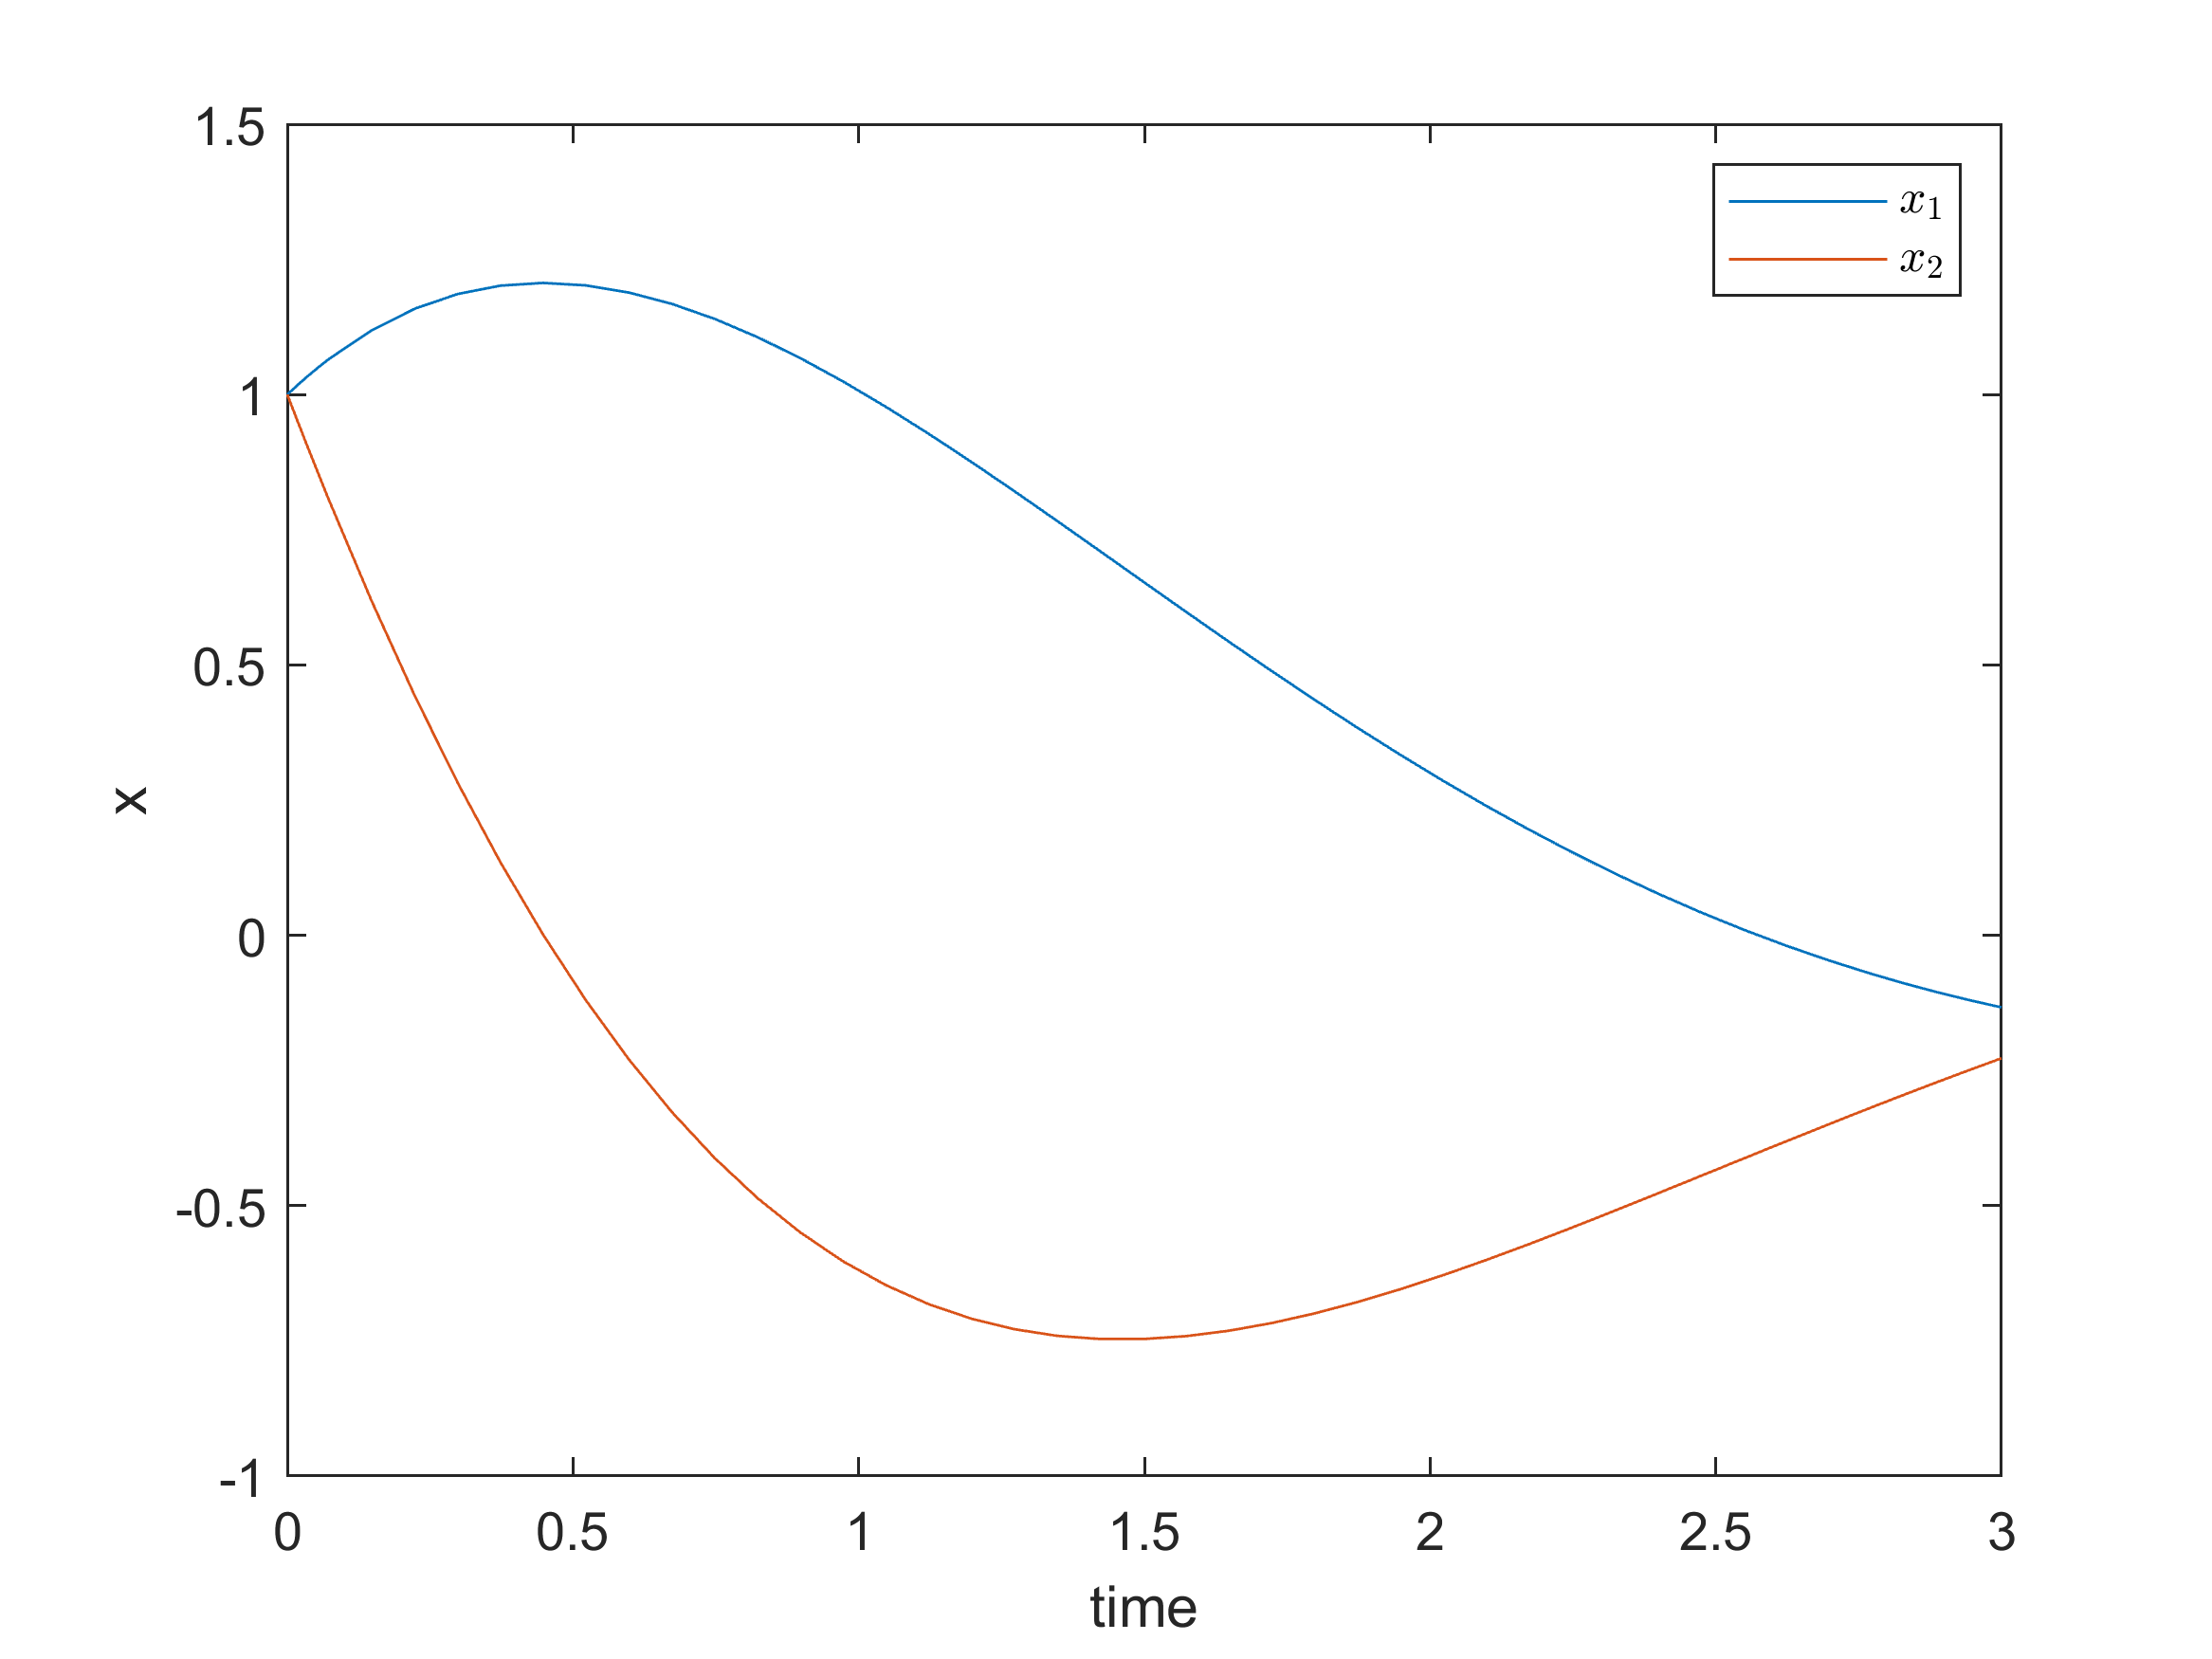
\includegraphics[width=12cm]{../Code/Q3/figures/xH1.png}
\end{figure}
	%%%%%%%%% H = 10I %%%%%%%%%
\item $H = 10I$
\begin{figure}[H]
	\caption{$K(t)$ in $H = 10I$}
	\centering
	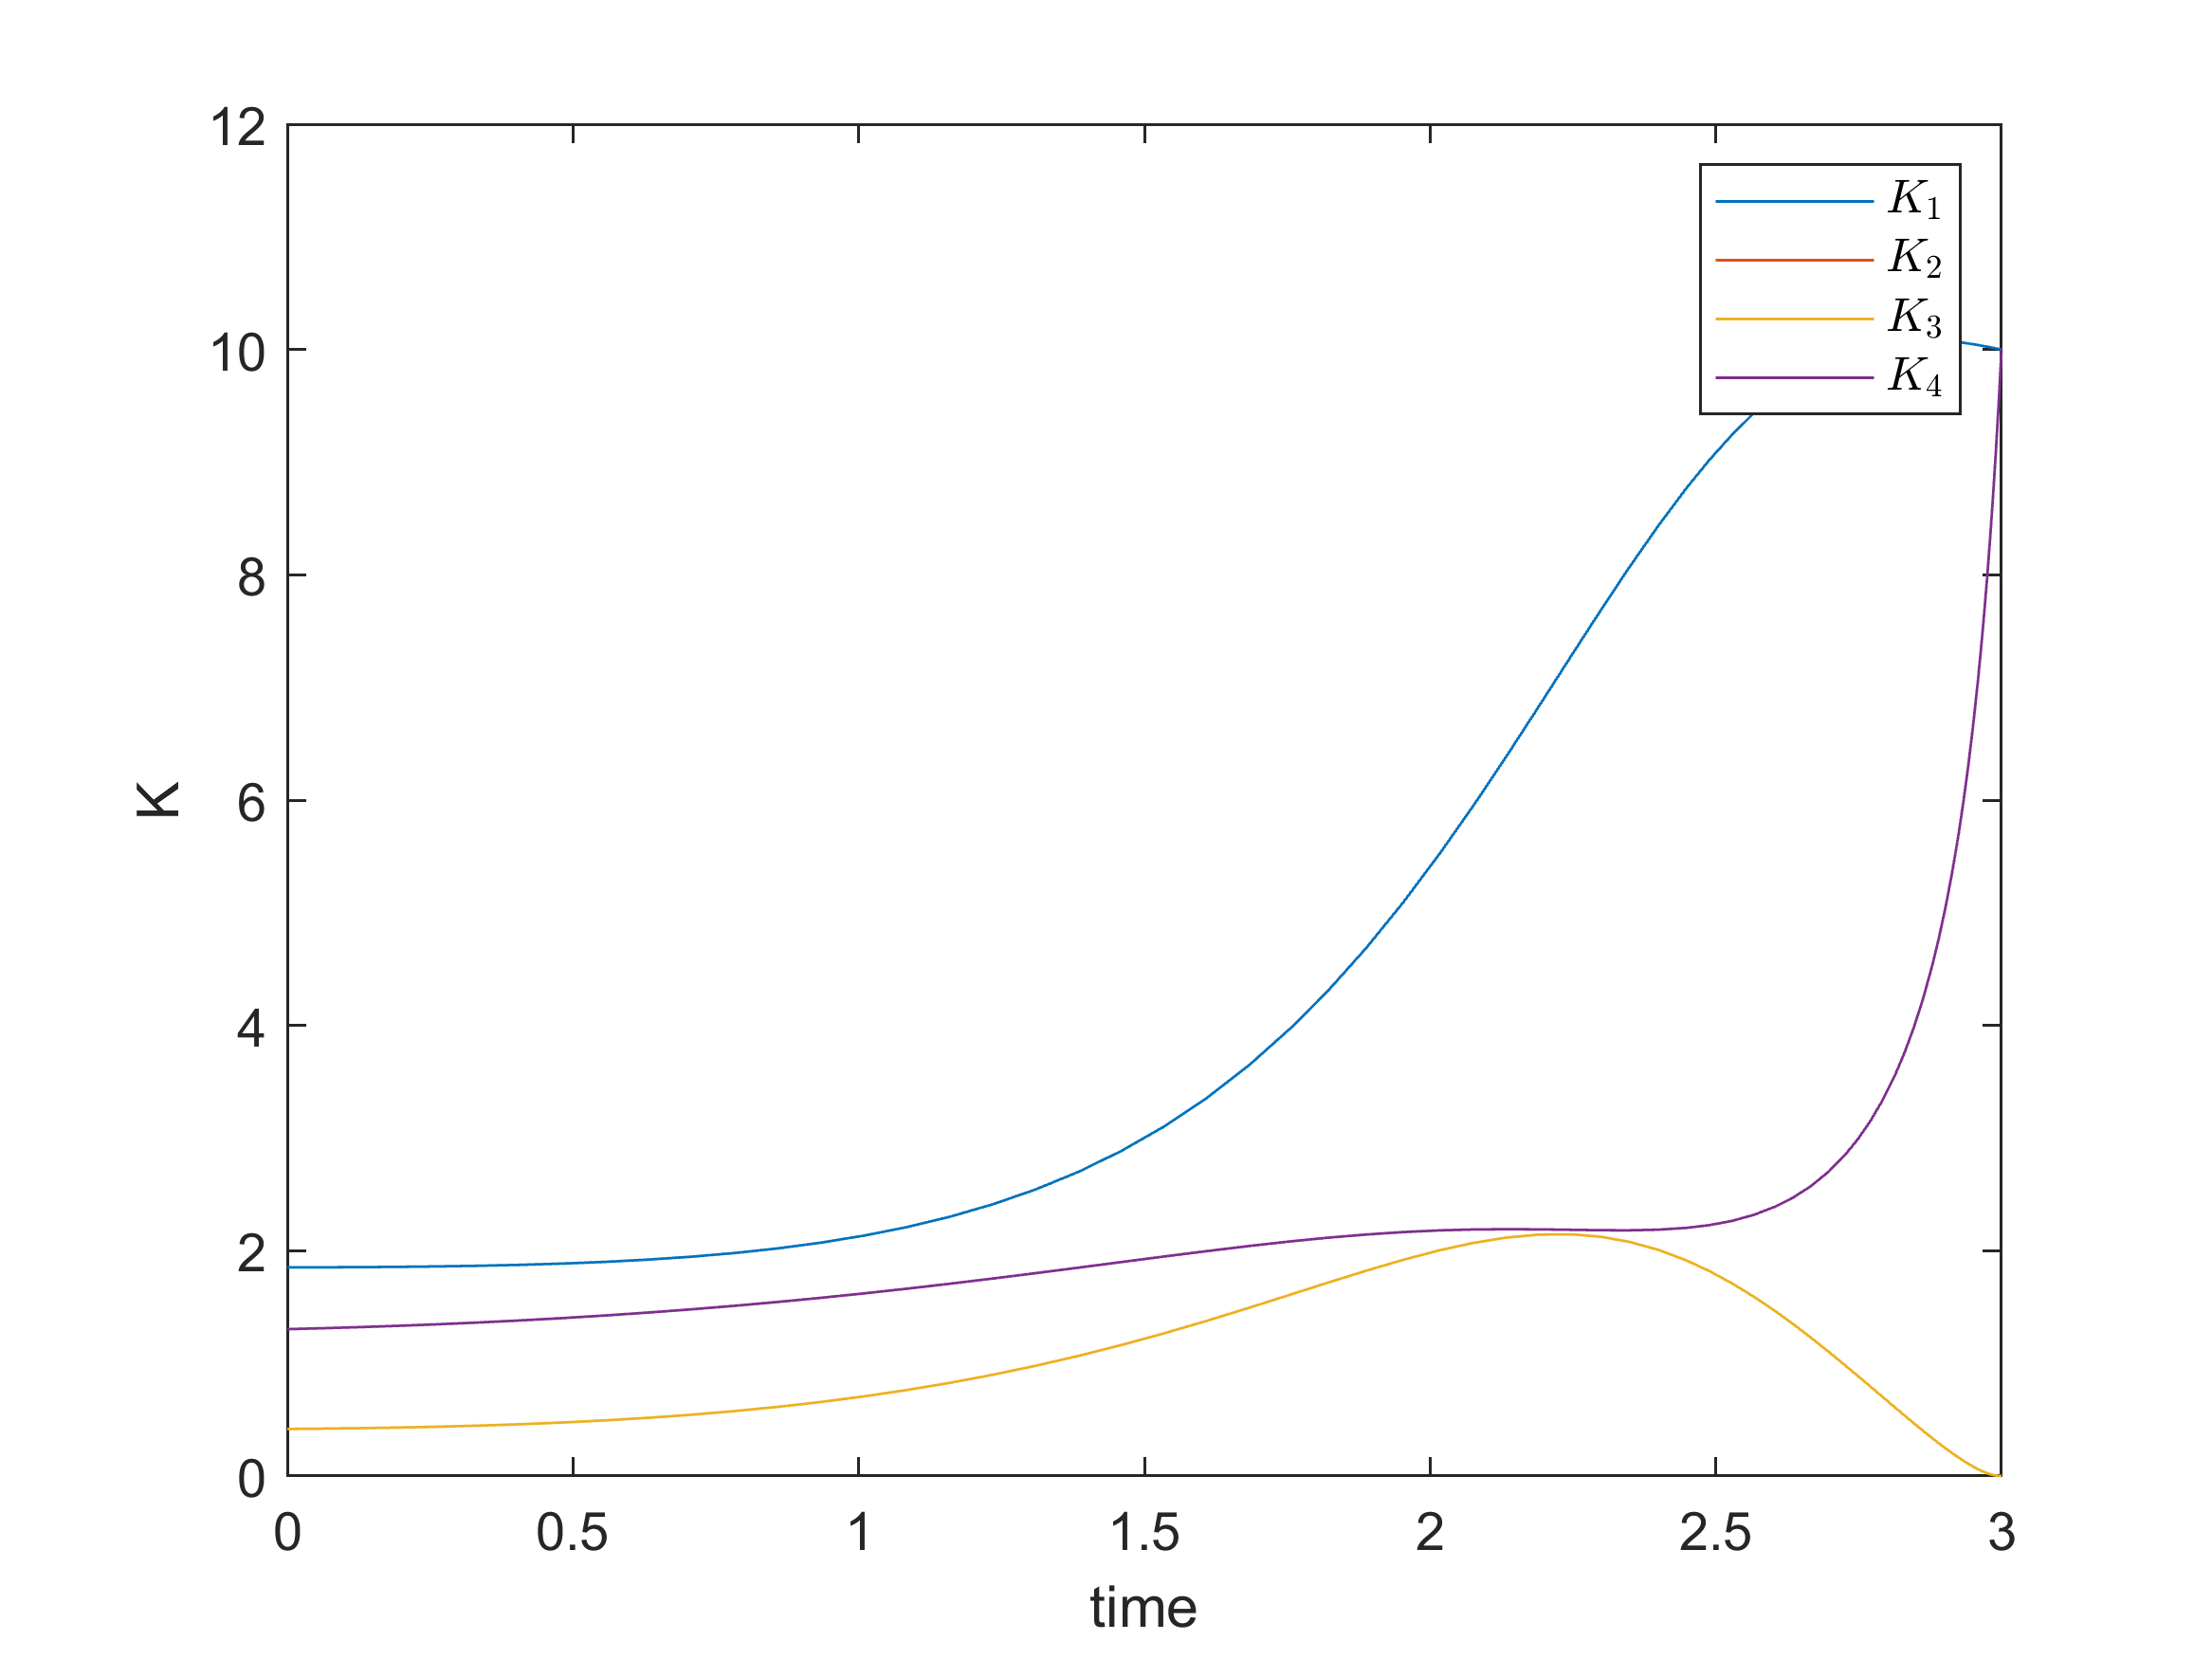
\includegraphics[width=12cm]{../Code/Q3/figures/KH10.png}
\end{figure}
\begin{figure}[H]
	\caption{$u(t)$ in $H = 10I$}
	\centering
	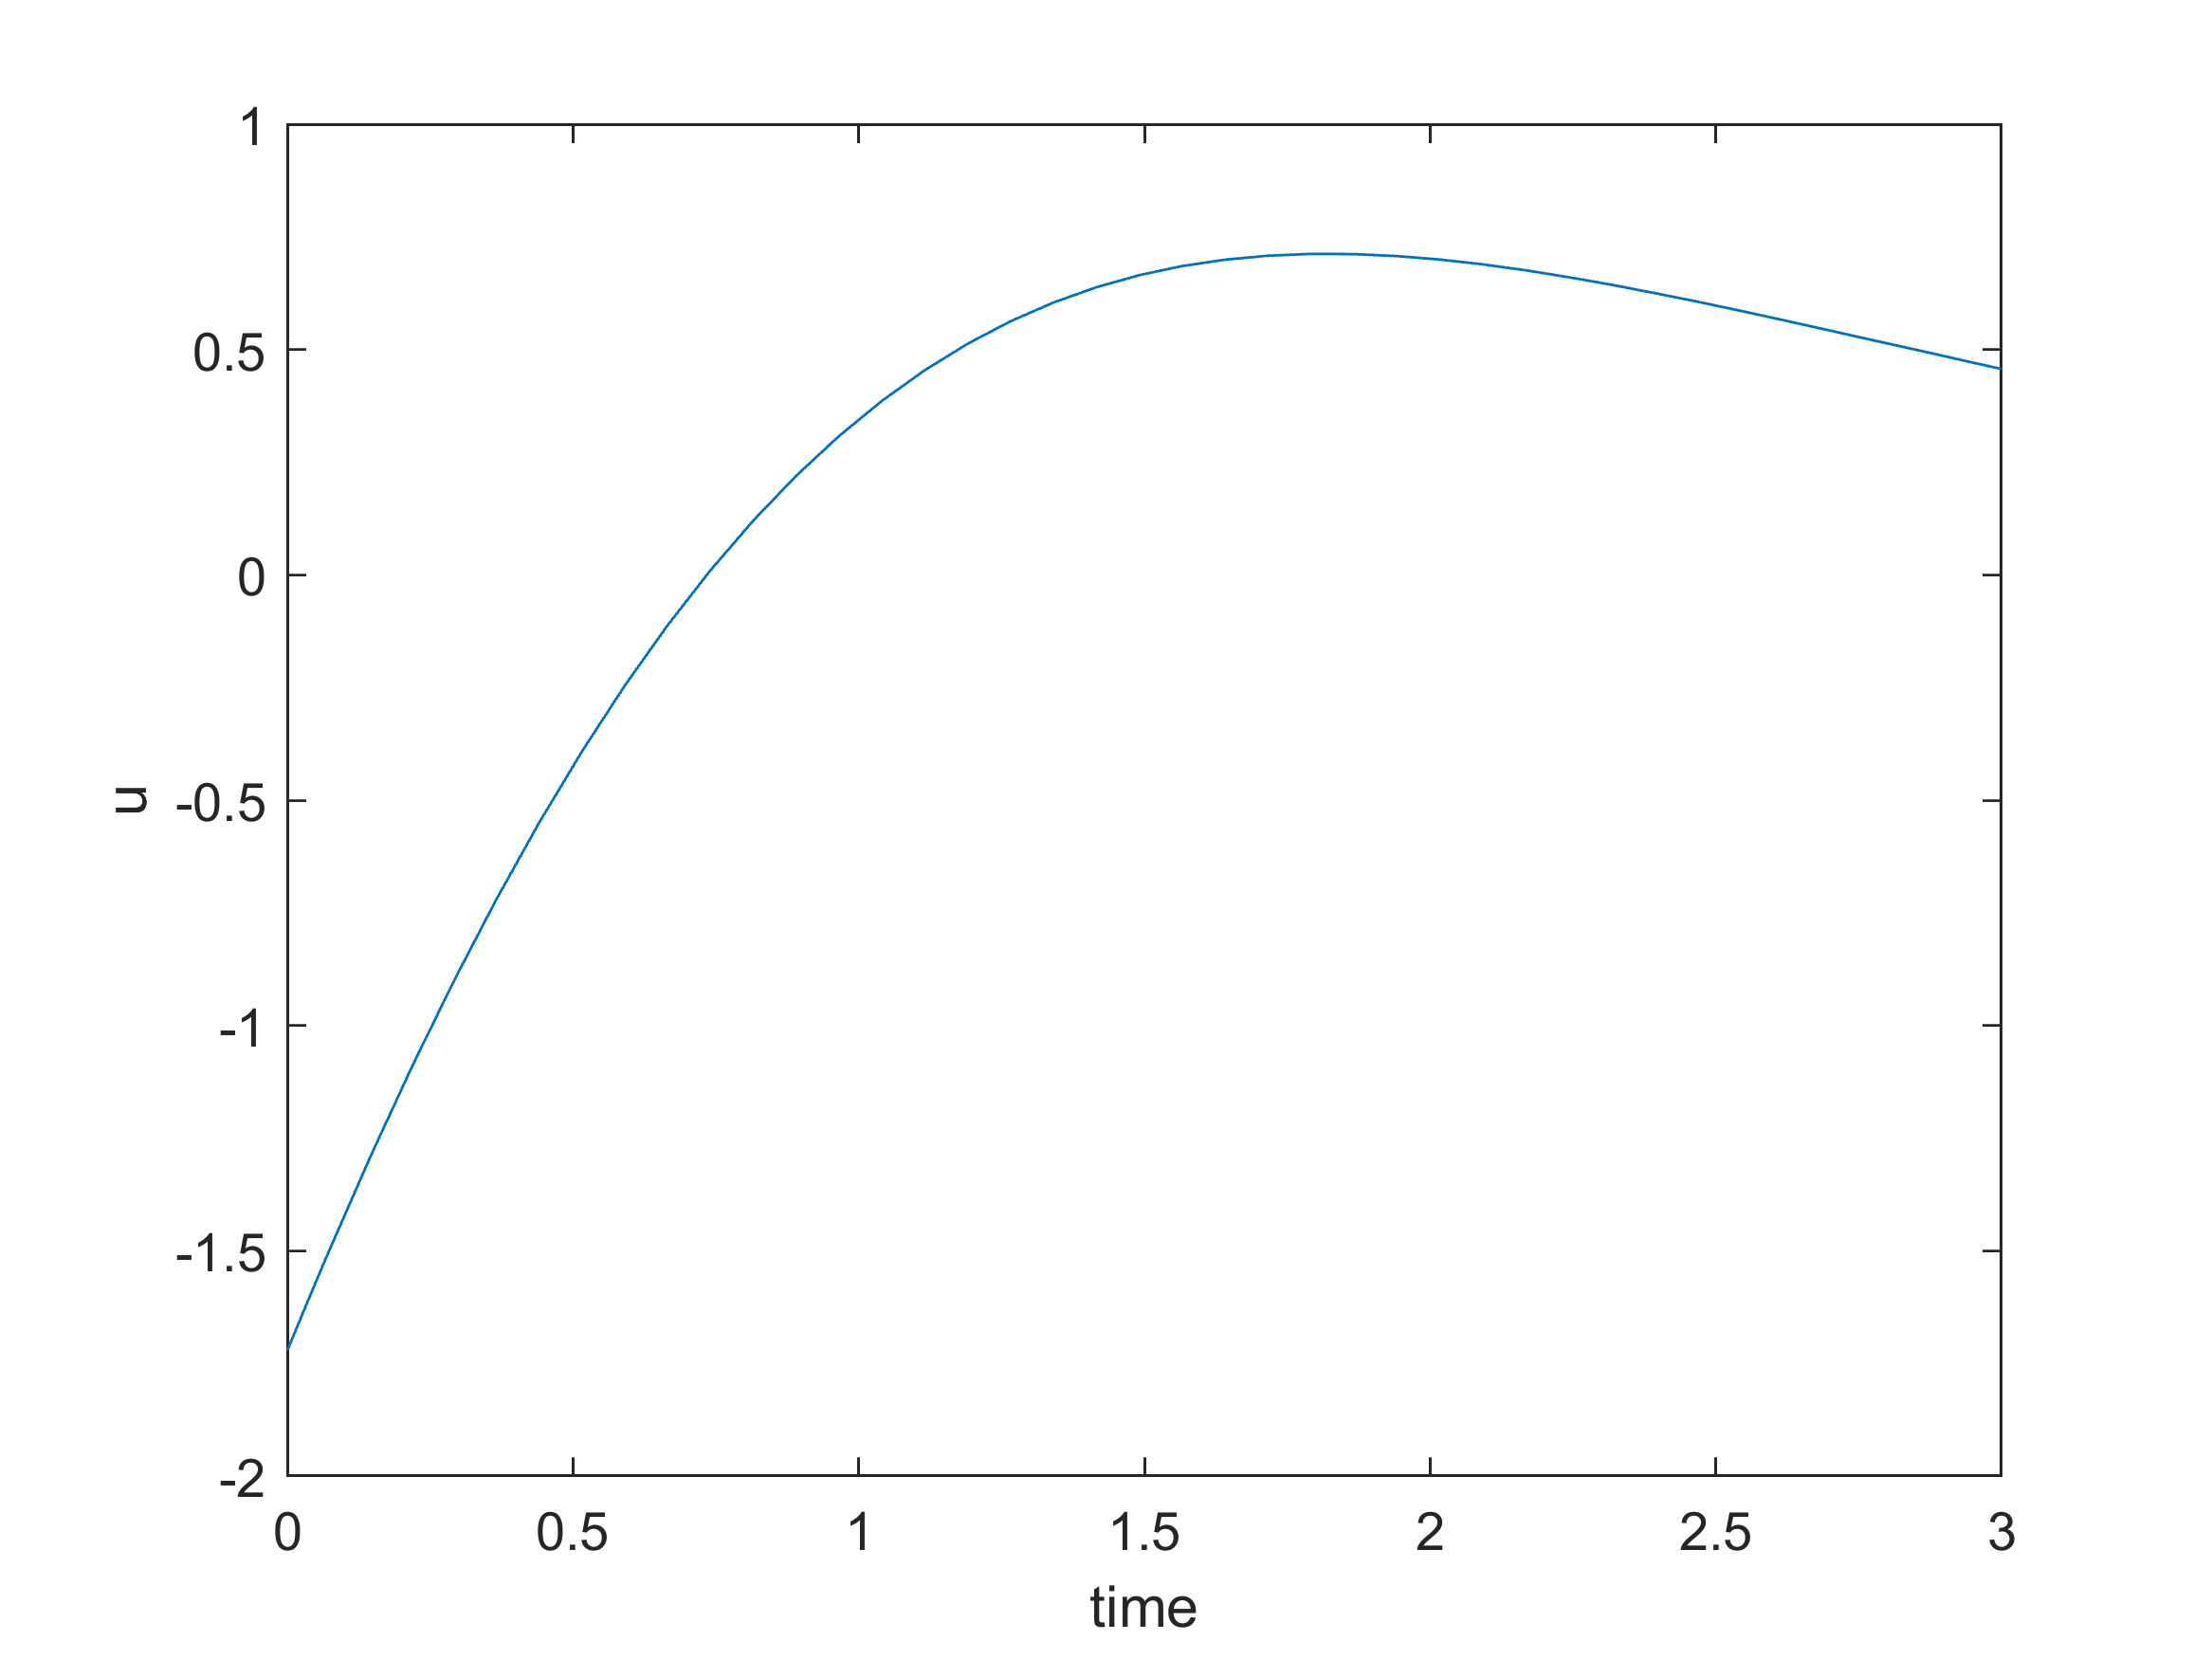
\includegraphics[width=12cm]{../Code/Q3/figures/uH10.png}
\end{figure}
\begin{figure}[H]
	\caption{System States $\vec x(t)$ in $H = 10I$}
	\centering
	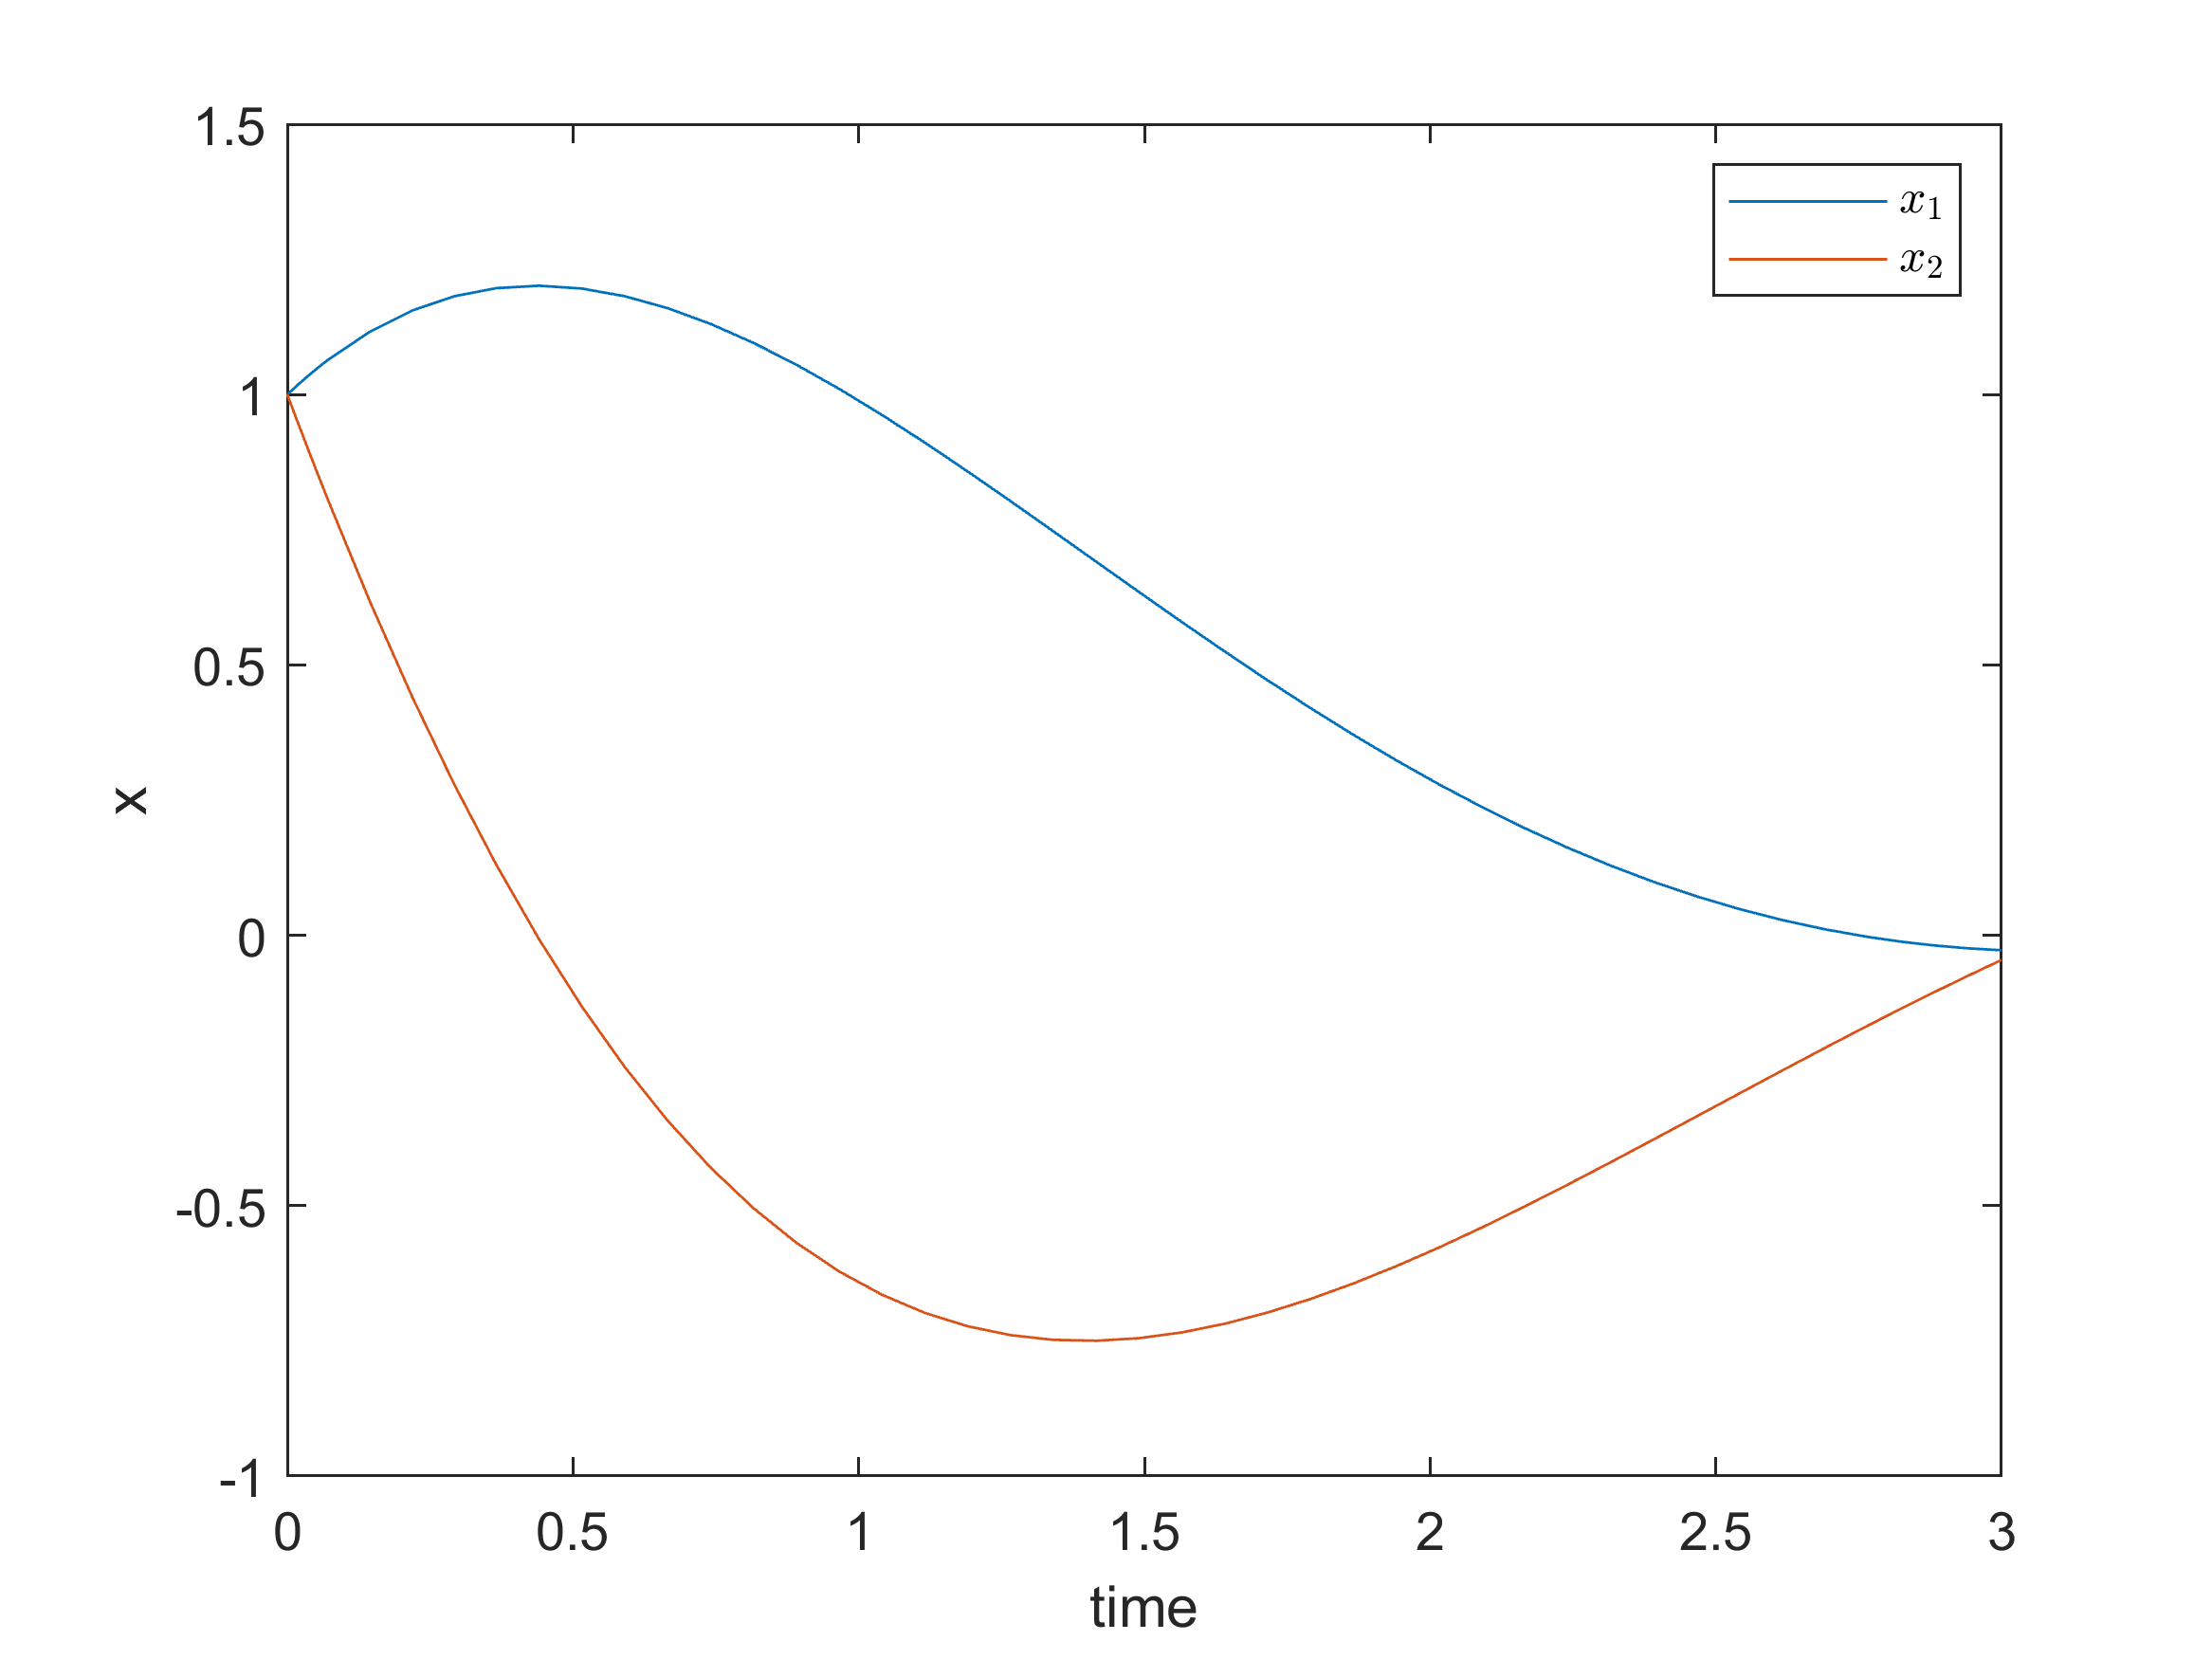
\includegraphics[width=12cm]{../Code/Q3/figures/xH10.png}
\end{figure}
	%%%%%%%%% H = 100I %%%%%%%%%
\item $H = 100I$
\begin{figure}[H]
	\caption{$K(t)$ in $H = 100I$}
	\centering
	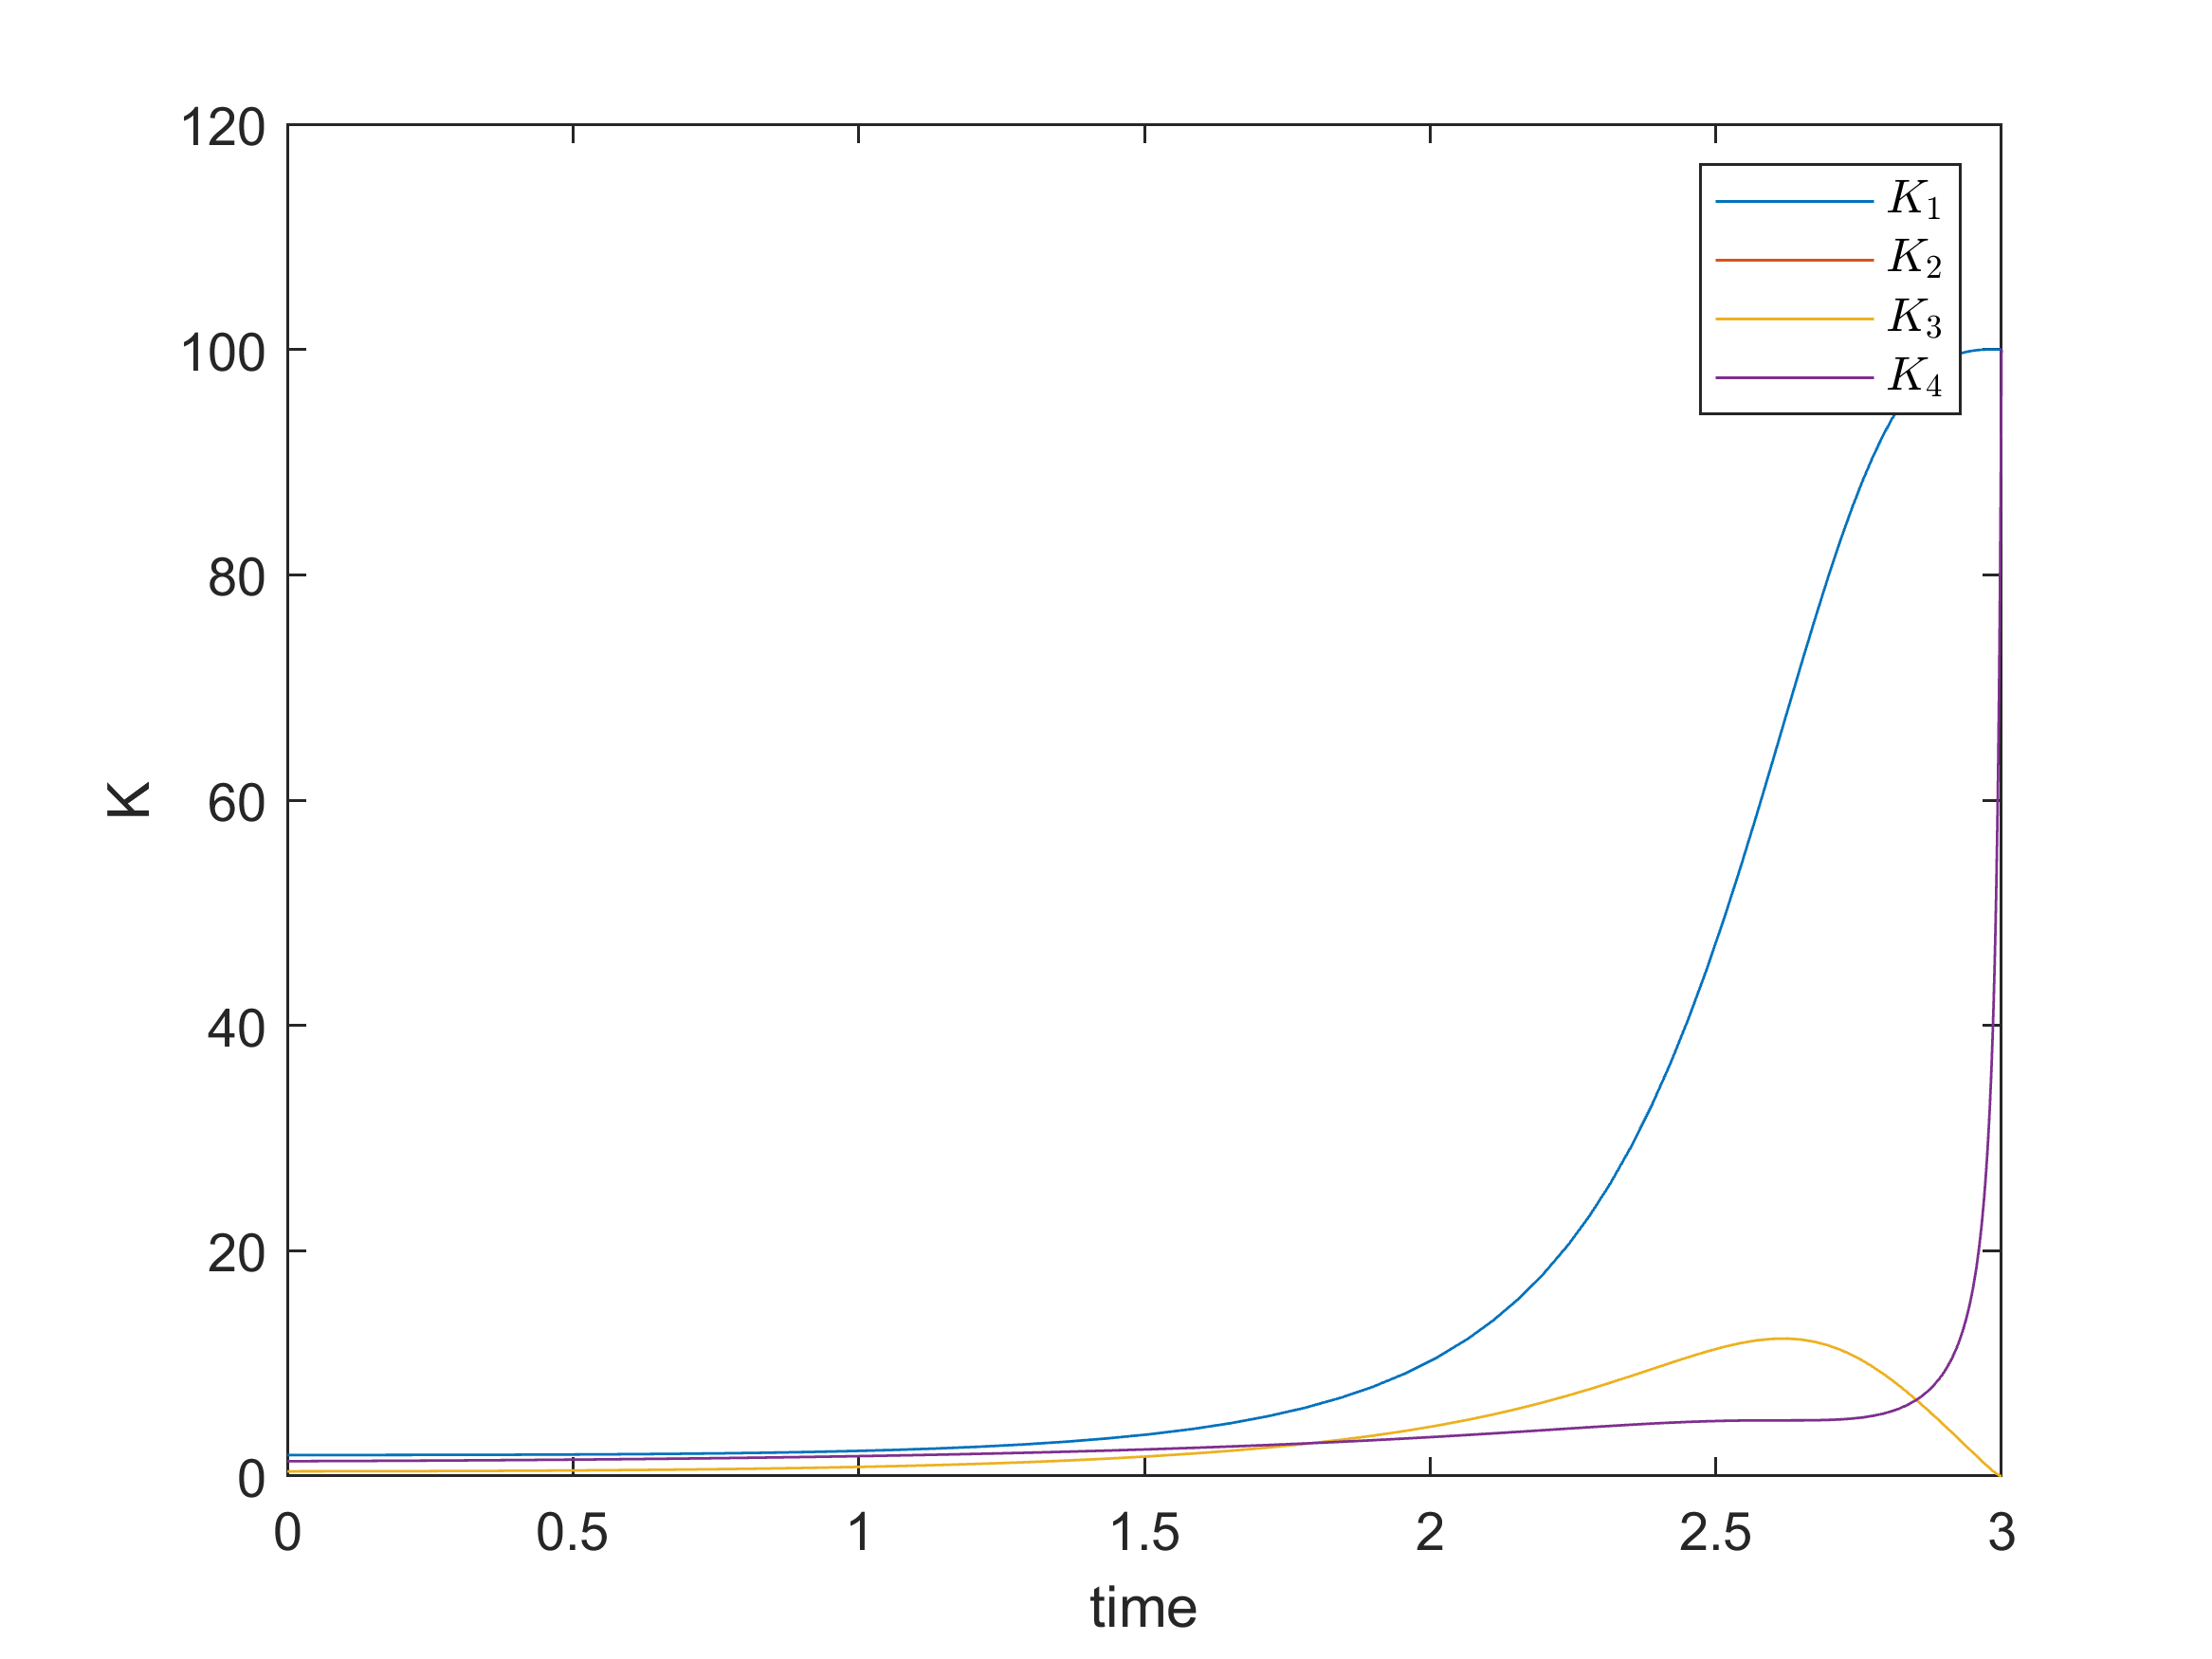
\includegraphics[width=12cm]{../Code/Q3/figures/KH100.png}
\end{figure}
\begin{figure}[H]
	\caption{$u(t)$ in $H = 100I$}
	\centering
	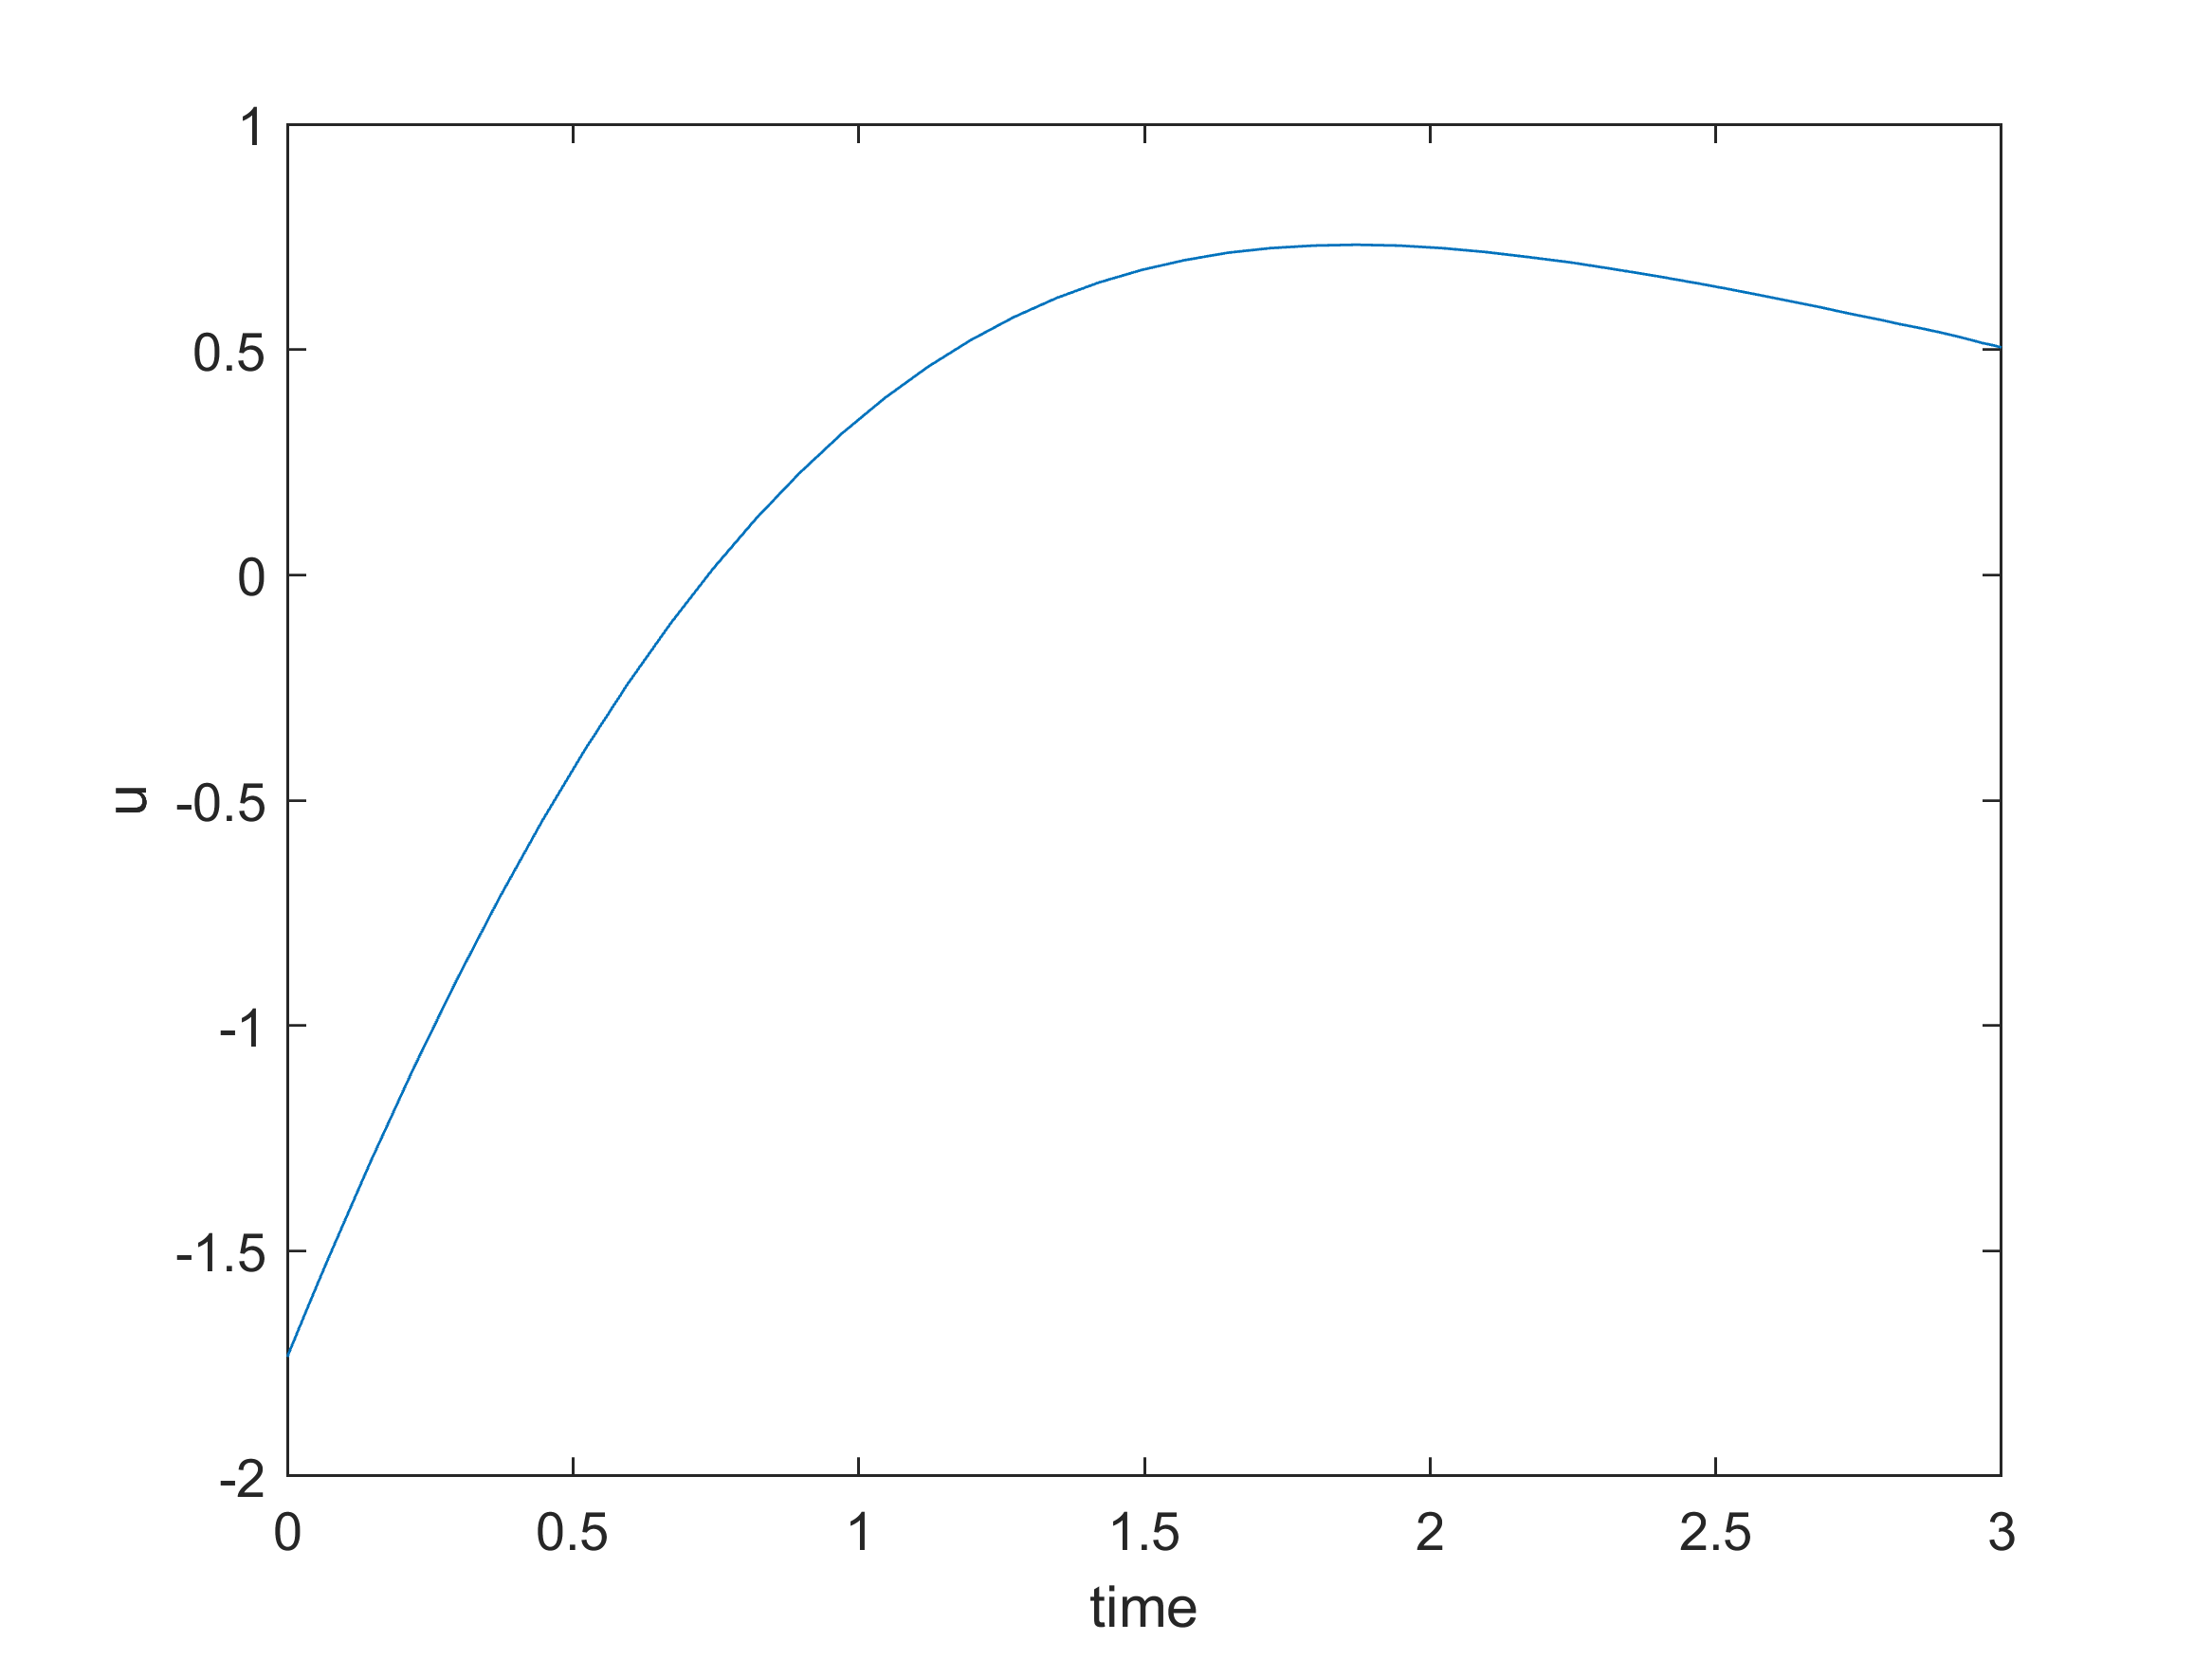
\includegraphics[width=12cm]{../Code/Q3/figures/uH100.png}
\end{figure}
\begin{figure}[H]
	\caption{System States $\vec x(t)$ in $H = 100I$}
	\centering
	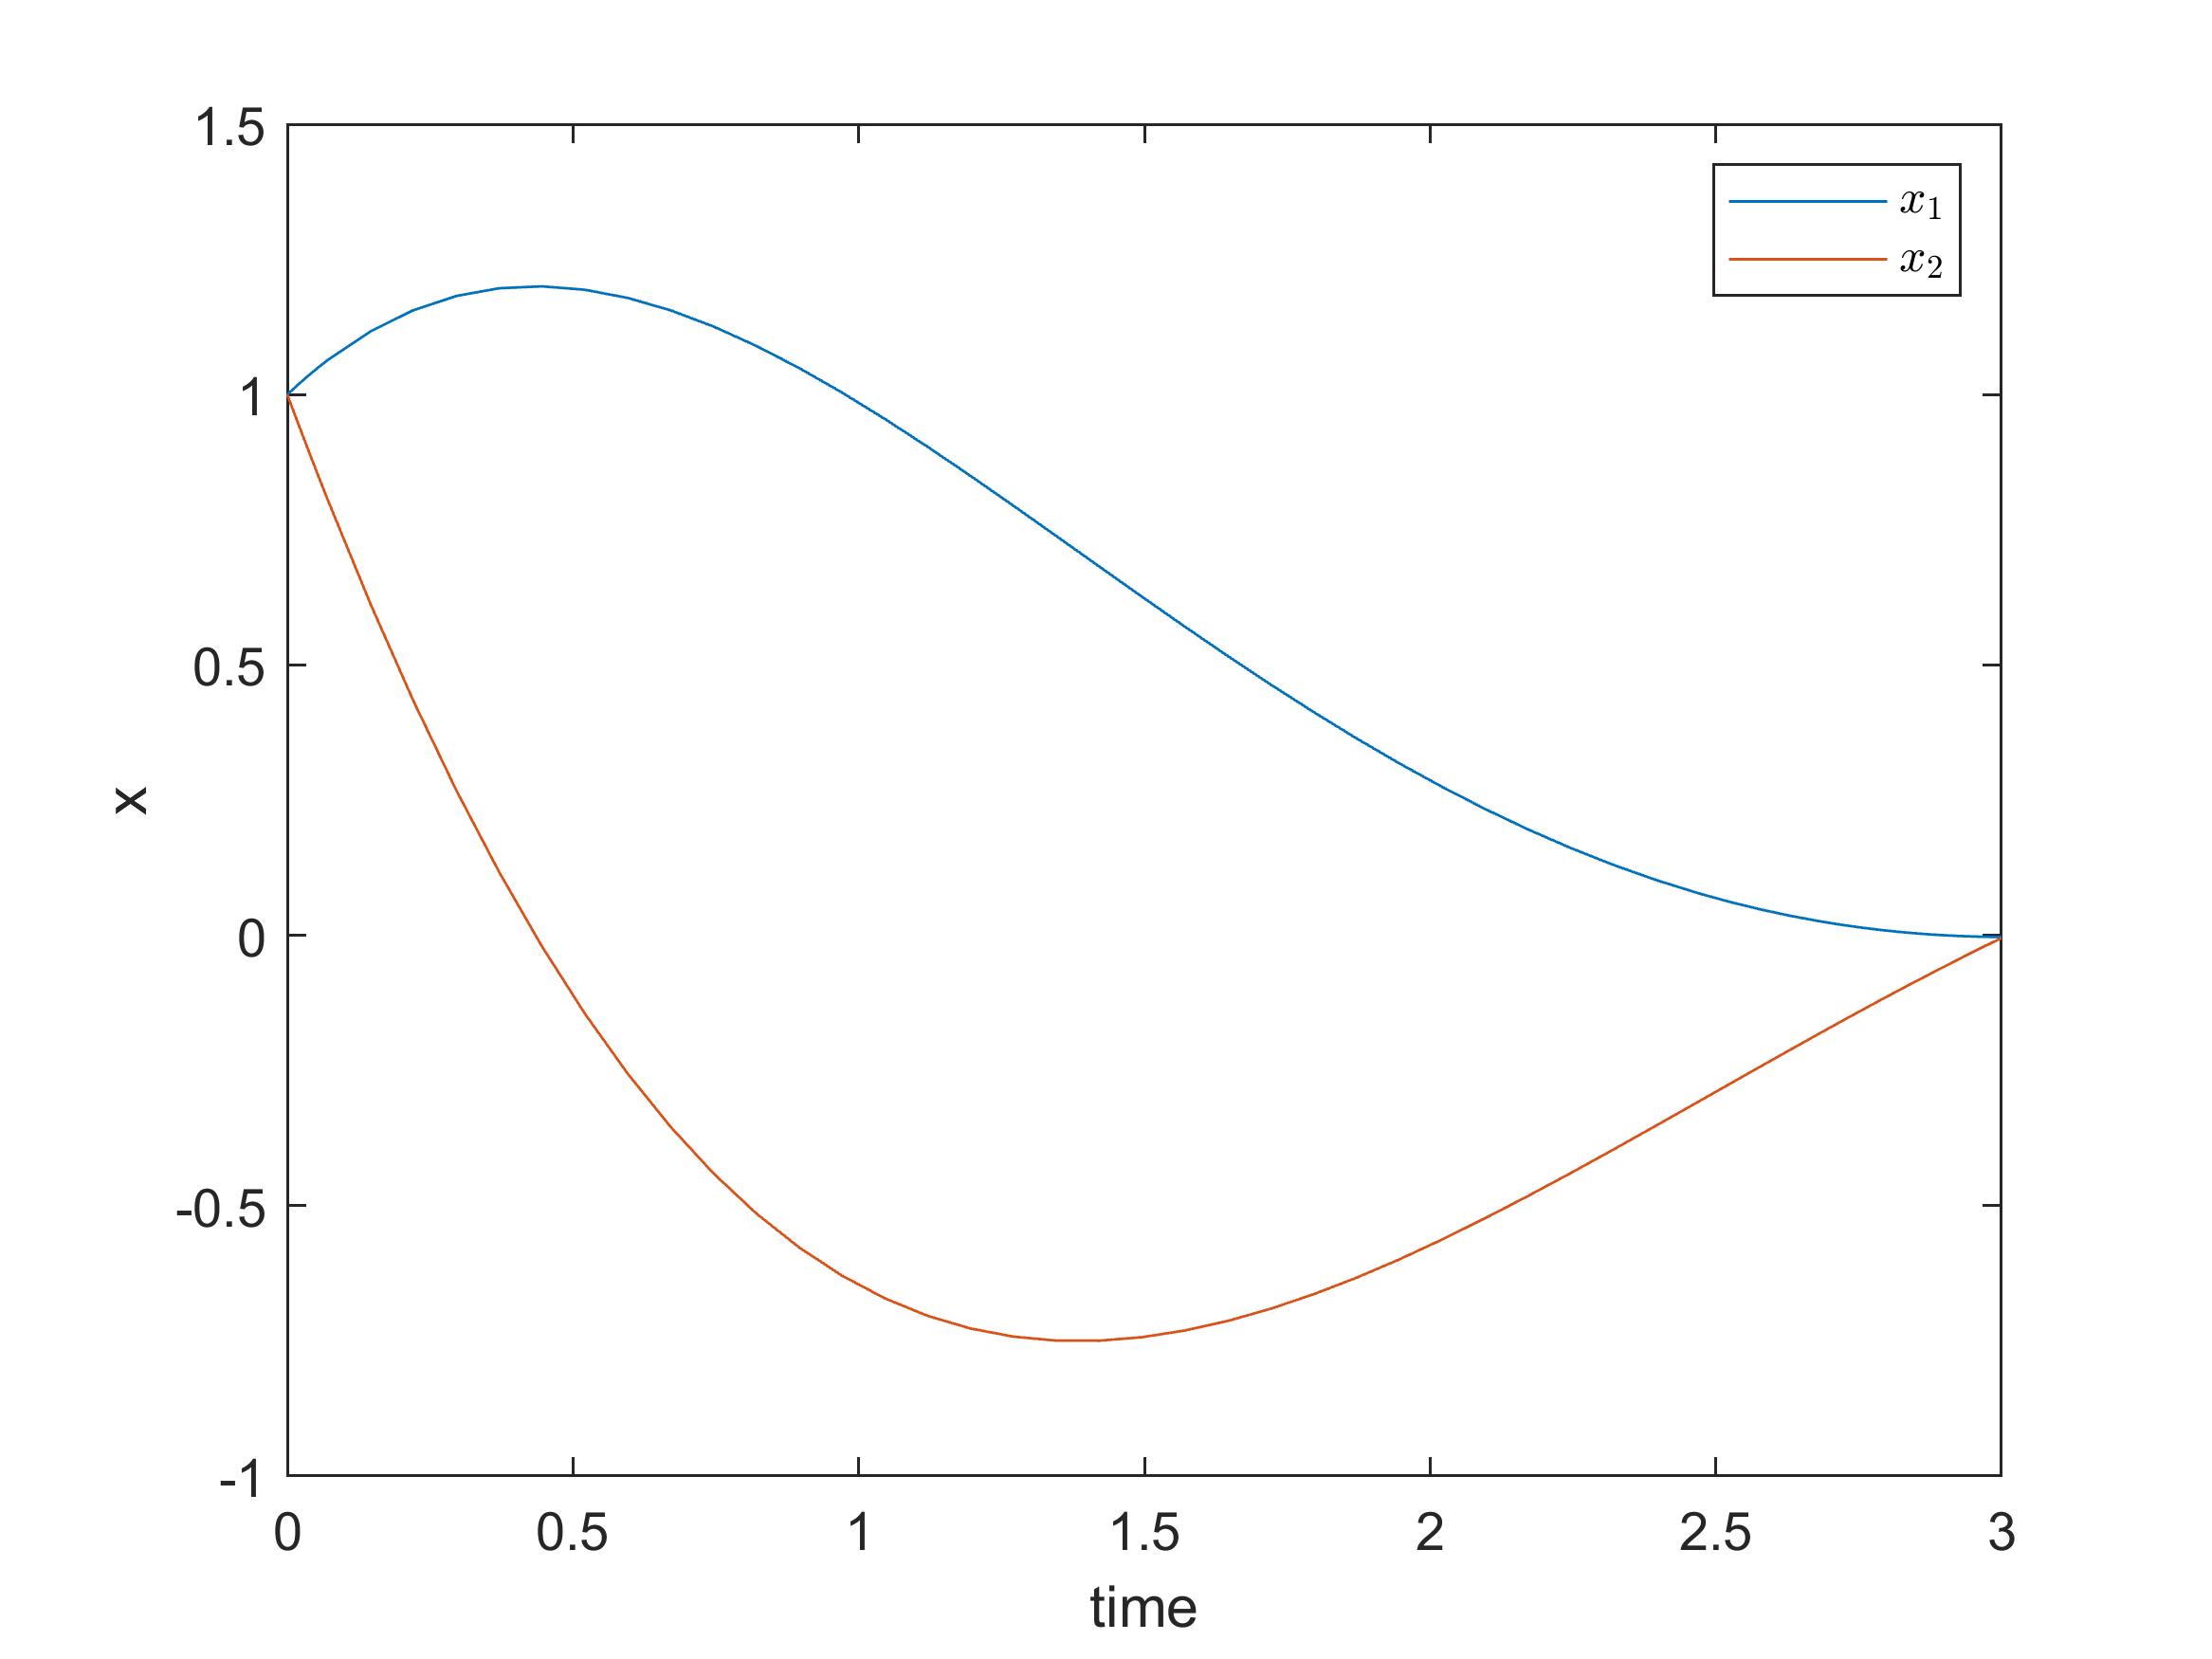
\includegraphics[width=12cm]{../Code/Q3/figures/xH100.png}
\end{figure}
%%%%%%%%% K(t) sub plot %%%%%%%%%
\item $K(t)$ for all simulated $H$
\begin{figure}[H]
	\caption{$K(t)$ for all simulated $H$}
	\centering
	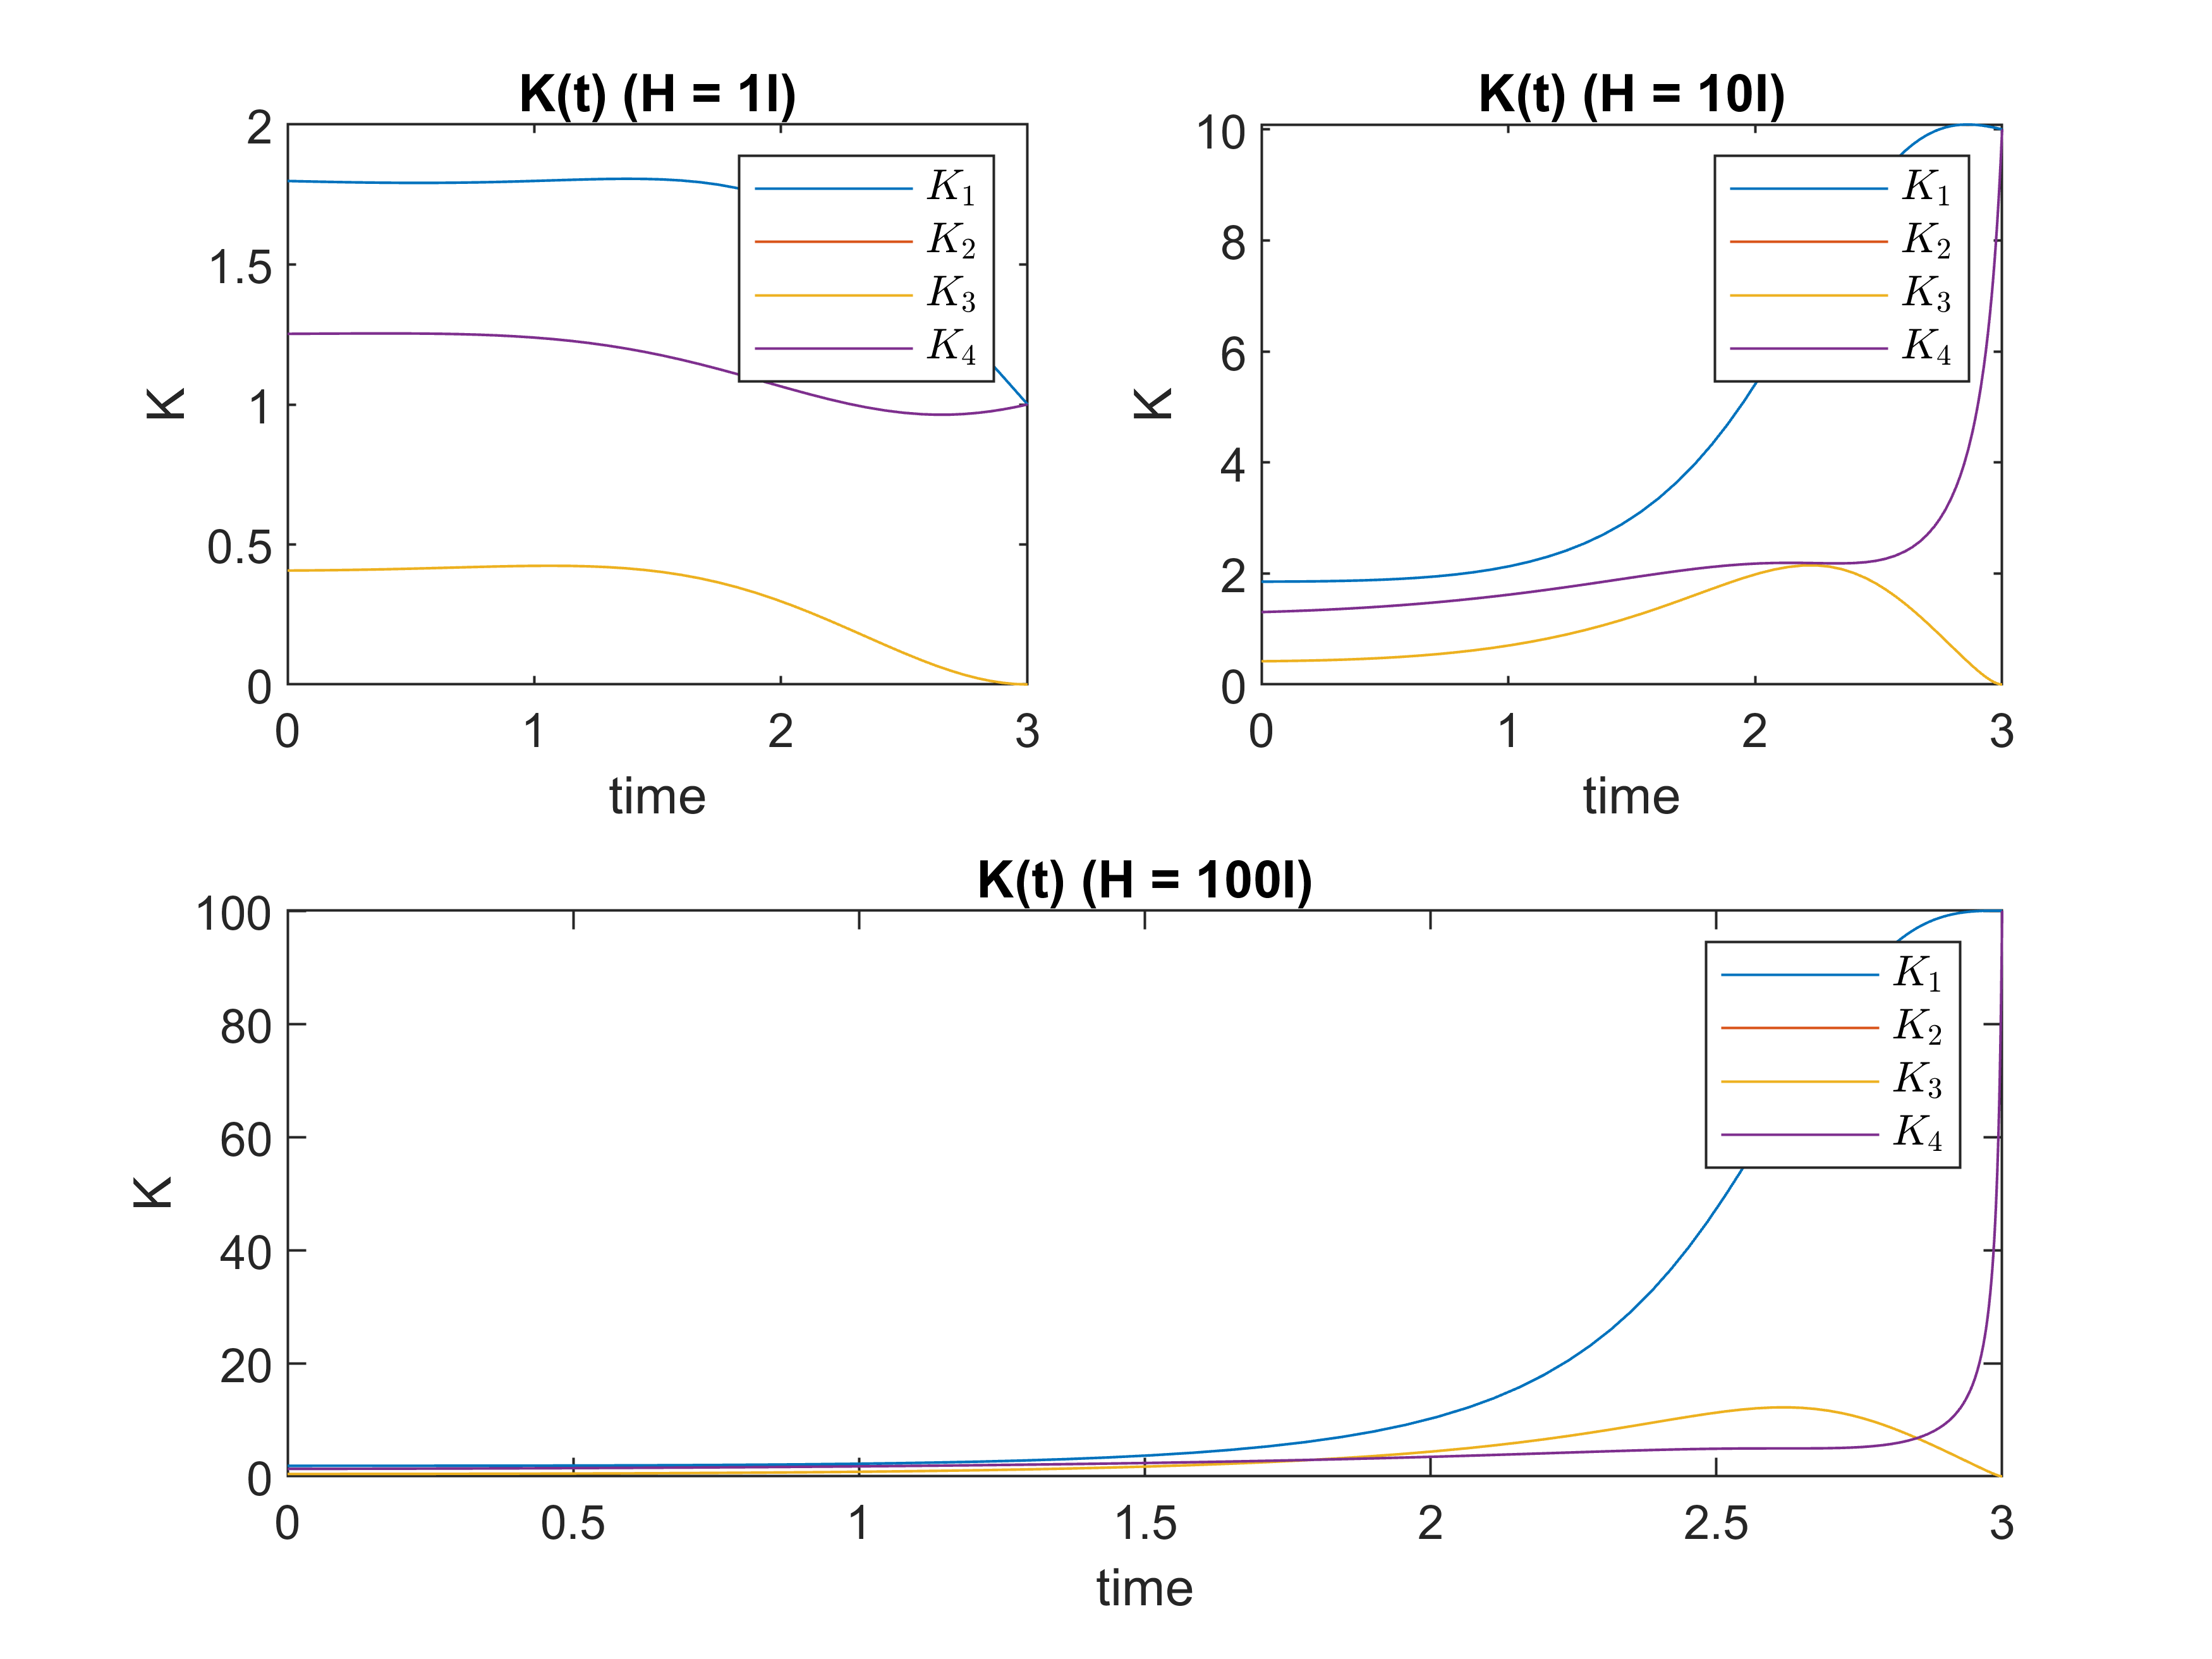
\includegraphics[width=12cm]{../Code/Q3/figures/SubplotQ3_cKII.png}
\end{figure}
%%%%%%%%% u(t) sub plot %%%%%%%%%
\item $u(t)$ for all simulated $H$
\begin{figure}[H]
	\caption{$u(t)$ for all simulated $H$}
	\centering
	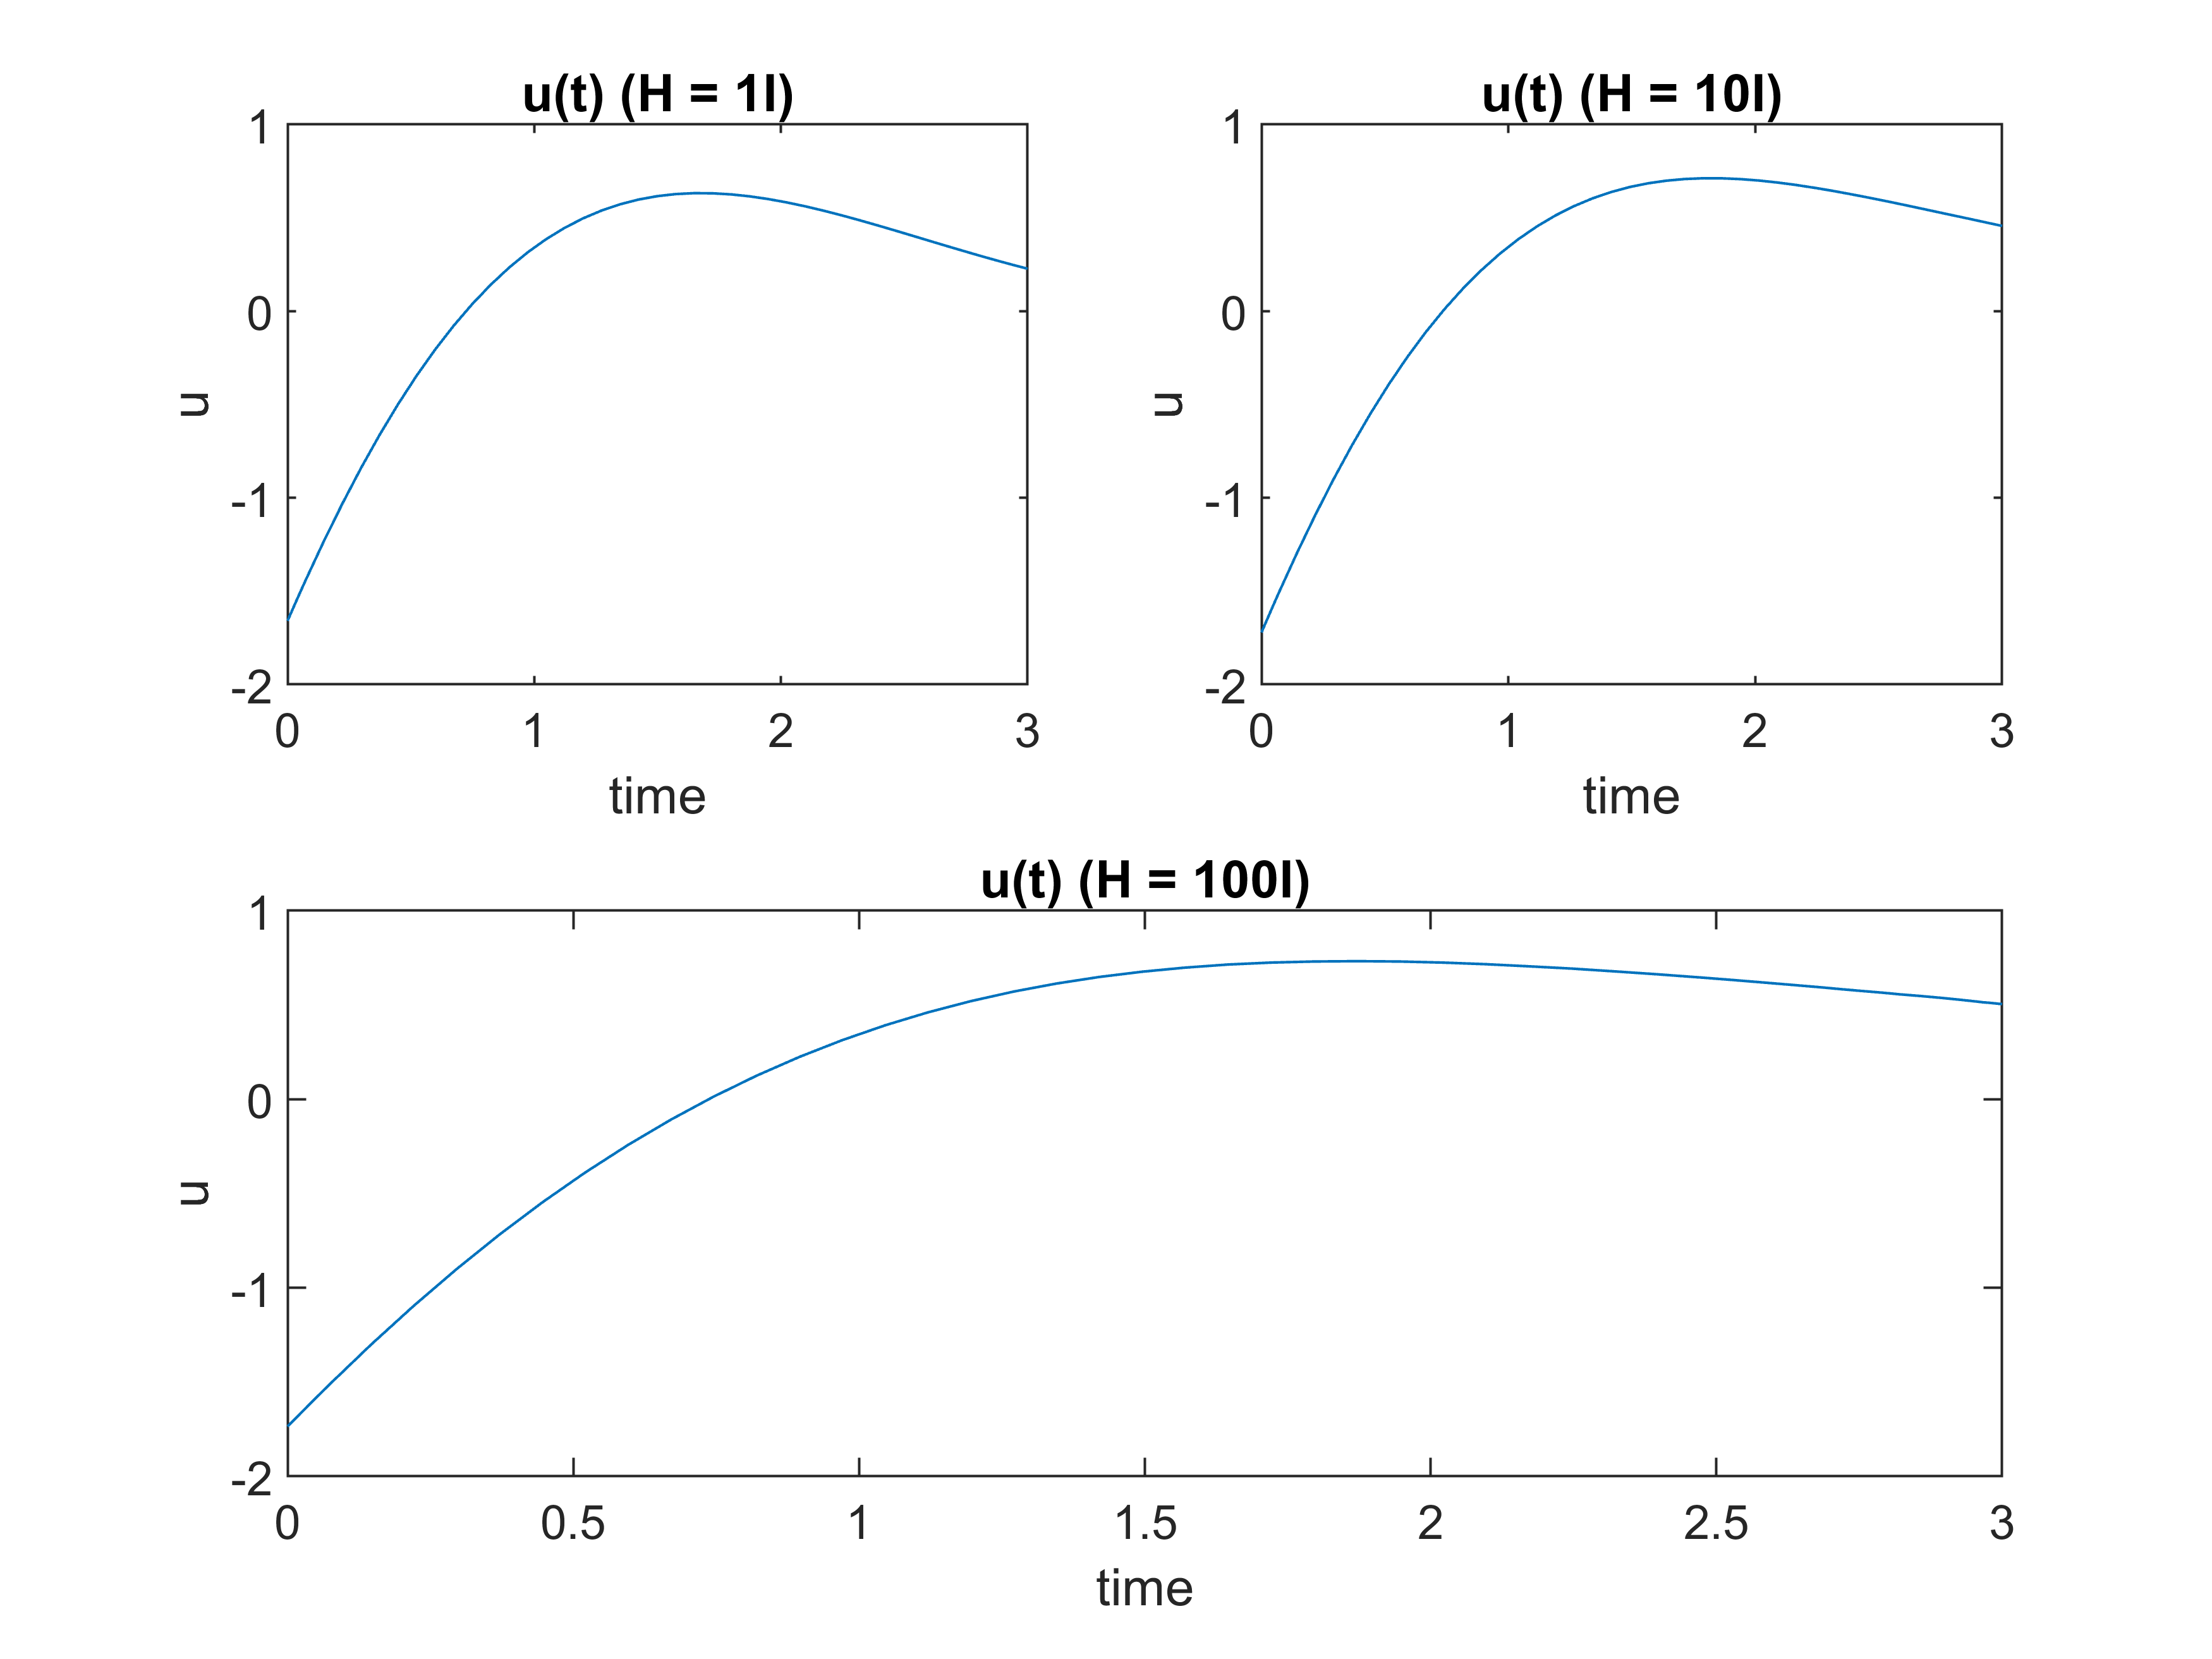
\includegraphics[width=12cm]{../Code/Q3/figures/SubplotQ3_cuII.png}
\end{figure}
%%%%%%%%% u(t) sub plot %%%%%%%%%
\item System States $\vec x(t)$ for all simulated $H$
\begin{figure}[H]
	\caption{System States $\vec x(t)$ for all simulated $H$}
	\centering
	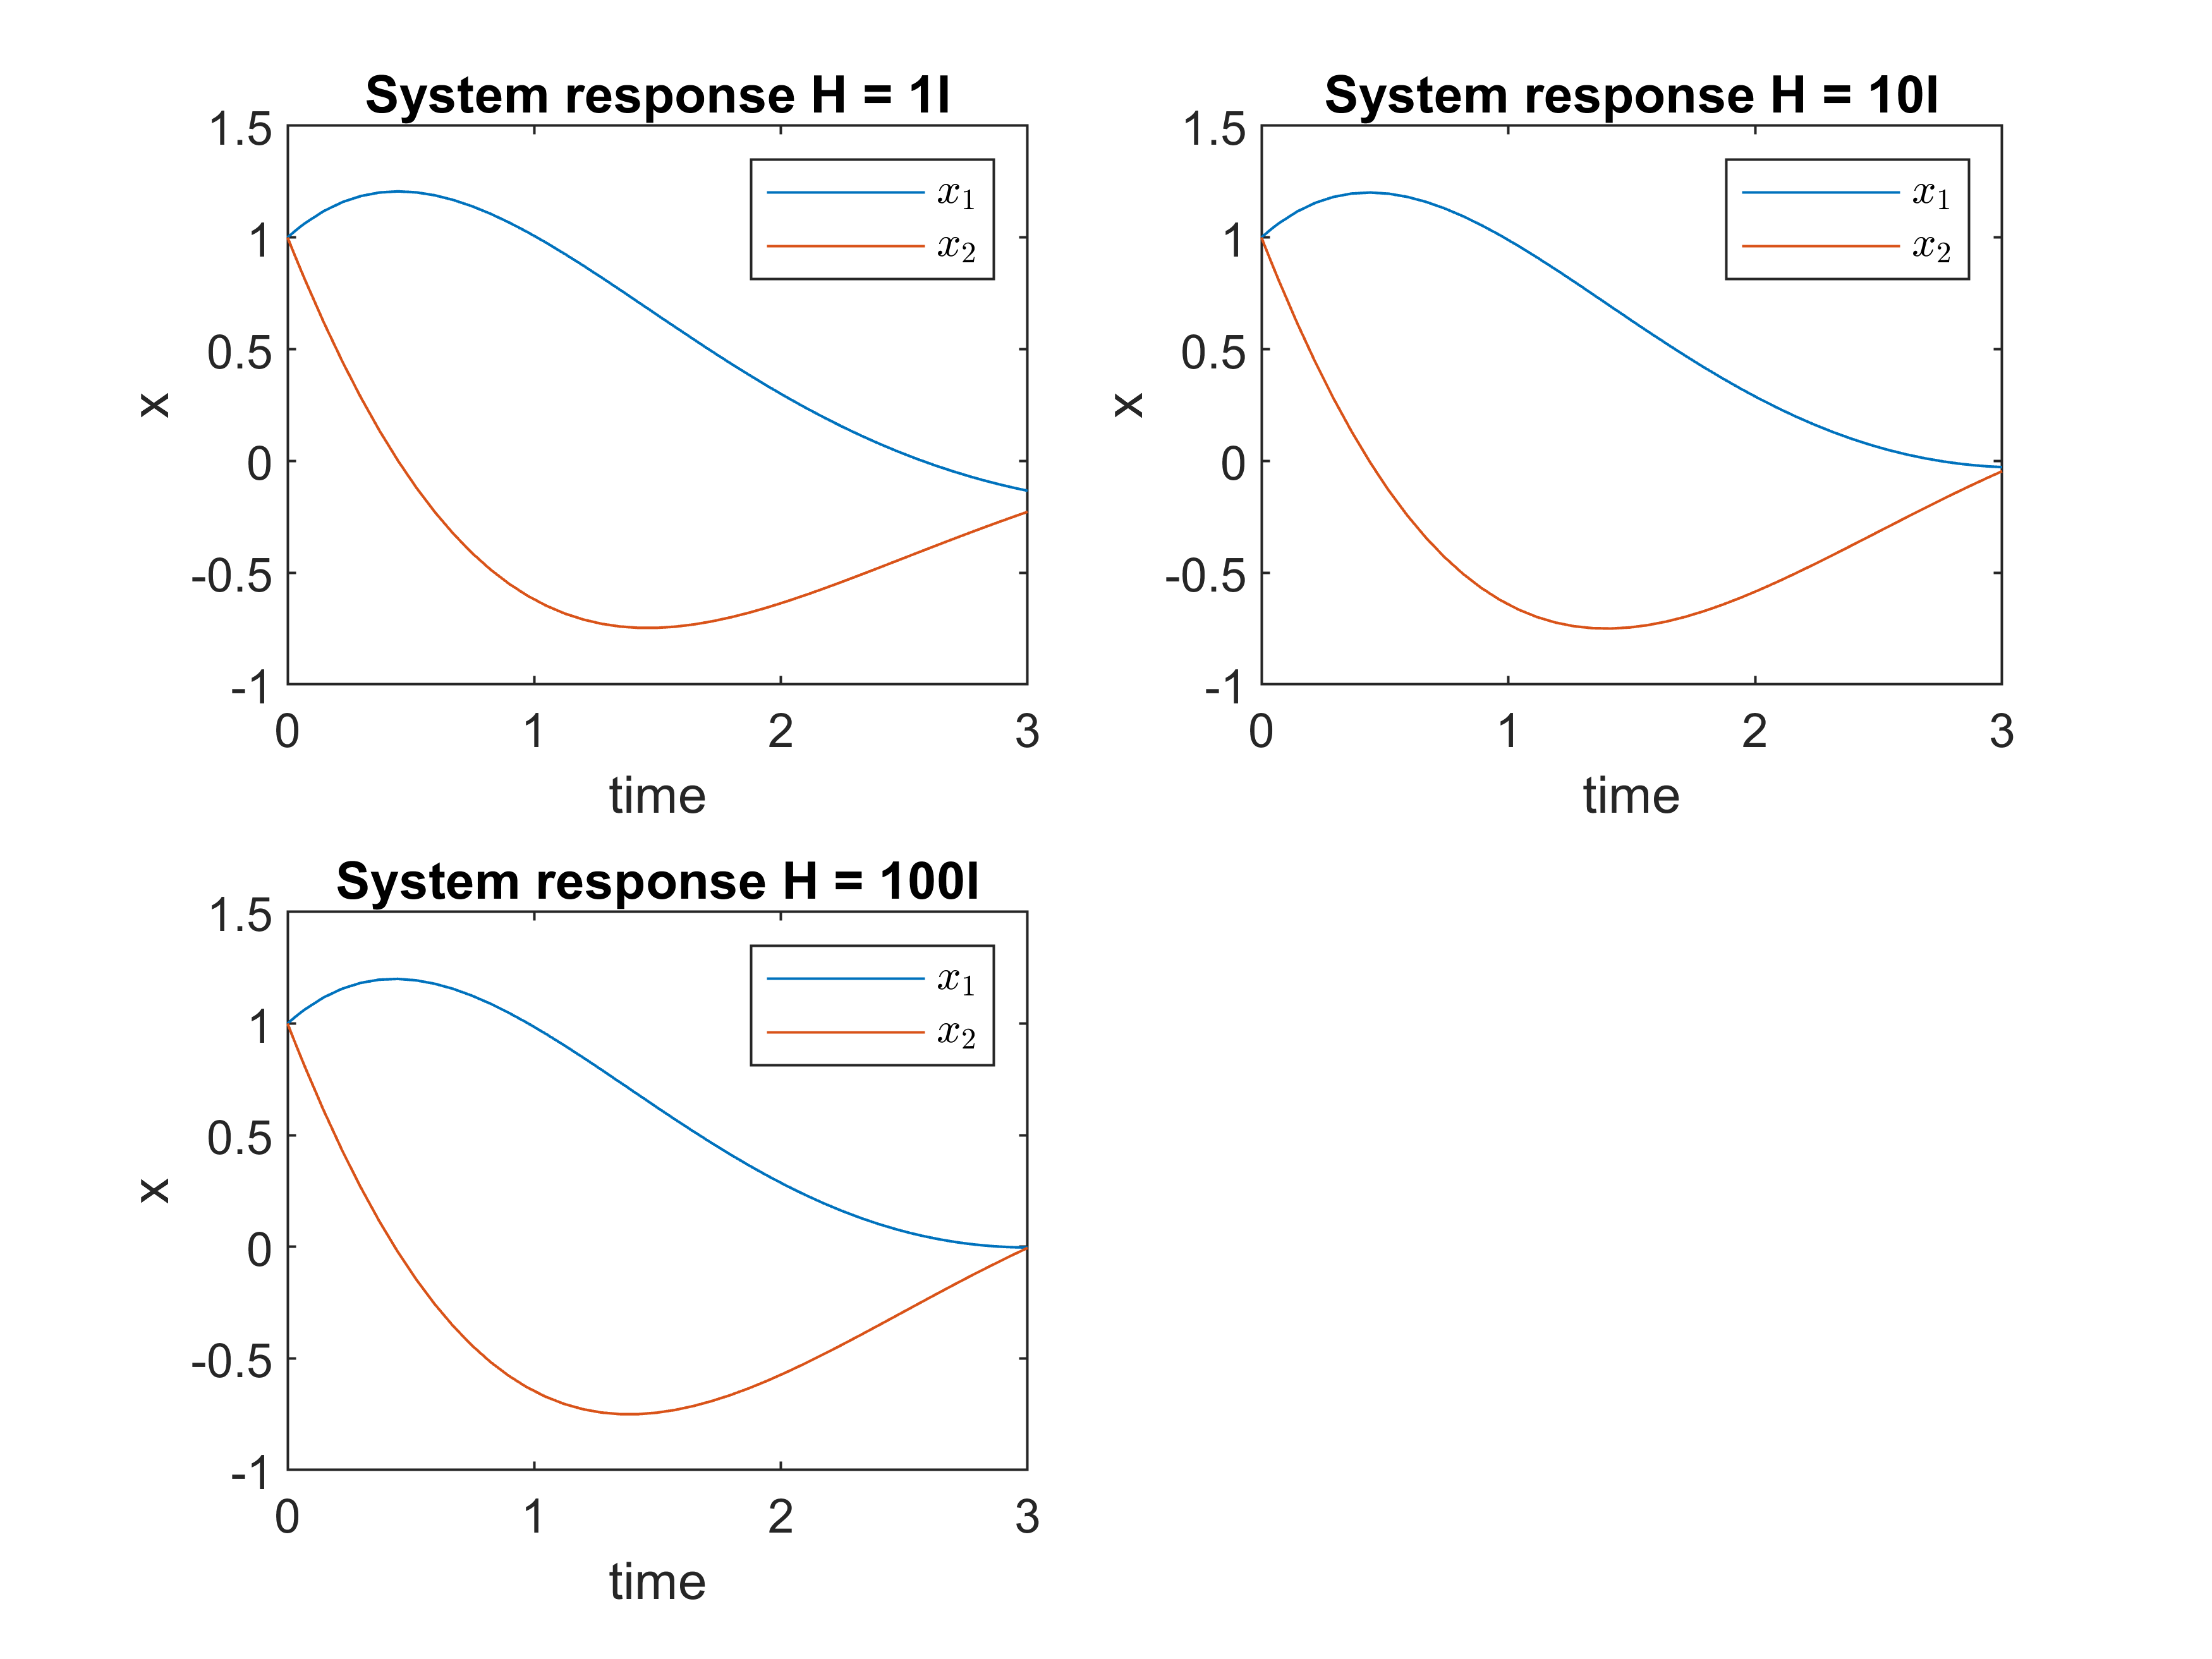
\includegraphics[width=12cm]{../Code/Q3/figures/SubplotQ3_cII.png}
\end{figure}
\end{itemize}